\documentclass[11pt]{article}

% ---------- Packages ----------
\usepackage[margin=1in]{geometry}
\usepackage{amsmath,amssymb,amsthm}
\usepackage{physics}
\usepackage{graphicx}
\usepackage{booktabs}
\usepackage{array}
\usepackage{caption}
\usepackage{subcaption}
\usepackage{hyperref}
\usepackage{authblk}
\usepackage{siunitx}
\usepackage{xcolor}
\usepackage[numbers,sort&compress]{natbib}
\usepackage{float}
\usepackage{enumitem}
\PassOptionsToPackage{hyphens}{url}
\usepackage[hyphens]{url}

\hypersetup{
  colorlinks=true,
  linkcolor=blue!50!black,
  citecolor=blue!50!black,
  urlcolor=blue!50!black
}

\title{\textbf{Robustness of Quantum Teleportation under Bell-Entangled Channels:\\
Noise and Routing-Overhead Analysis with Error Mitigation via Linear Zero-Noise Extrapolation}}

\author[1]{Fatima Aftab}
\author[1]{Laraib Bibi}
\author[1]{Sara Masood}
\author[1]{Muhammad Shahan}
\affil[1]{School of Natural Sciences (SNS), National University of Sciences and Technology (NUST)}
\date{August 2026\\[0.3em]\normalsize Quantum Internship, Summer 2026, Group 5\\ Supervisor: Prof.\ Dr.\ Shahid Iqbal \quad Mentors: Ali, Tooba, Osaid}

\begin{document}

\maketitle

\begin{abstract}
\noindent
Quantum teleportation is a core primitive for quantum networks, but on real, noisy intermediate-scale quantum (NISQ) hardware its fidelity is degraded both by intrinsic noise channels and by compiler-inserted SWAP gates required when interacting qubits are not physically adjacent. The relative size of these two effects, and the extent to which the second can be mitigated in software, has not been established for this specific circuit-level setting. We simulate quantum teleportation under four standard single-qubit noise channels (bit-flip, phase-flip, depolarizing, amplitude-damping), derive closed-form fidelity expressions for each from the general noisy-teleportation superoperator, and separately quantify routing-induced fidelity loss by comparing a connectivity-respecting (``natural'') qubit layout against a layout that forces an extra SWAP gate (``forced''), using real calibration data from a 127-qubit IBM Eagle-family processor (\texttt{FakeSherbrooke}). We then apply Linear Zero-Noise Extrapolation (ZNE) via unitary gate folding to mitigate the worst-performing case. Among the three Pauli-type channels, bit-flip and phase-flip prove most damaging on average, contrary to an initial literature-based expectation that depolarizing and amplitude-damping noise would dominate; this ordering is explained analytically. Once noise is tied to a physically motivated hardware mechanism, forced routing produces a statistically significant $1.41\%$ fidelity drop relative to the natural layout ($z\approx14.70$), smaller than the $2.33\%$ drop predicted by a calibration-only two-qubit-gate model, because single-qubit gate error, readout error, and decoherence form a shared baseline that dilutes the relative comparison between layouts even as it lowers absolute fidelity in both. Linear ZNE recovers approximately $2.3$ percentage points of the fidelity lost to the forced layout ($0.9476\to0.9701$), cross-validated against a quadratic Lagrange extrapolation ($0.9723$, $\approx0.2\%$ deviation). These results indicate that routing overhead, not Bell-state choice, is the dominant hardware-limited error source in this setting, and that its impact is smaller in practice than a calibration-only estimate suggests once the full device noise model is taken into account -- with software-level error mitigation recovering a meaningful share of the residual loss.
\end{abstract}

\vspace{0.5em}
\noindent\textbf{Keywords:} quantum teleportation, Bell states, noise channels, qubit routing, SWAP overhead, zero-noise extrapolation, NISQ

\section{Introduction}

Quantum teleportation \citep{bennett1993} transfers an unknown single-qubit state between two parties using a shared maximally entangled pair (a Bell state) and two bits of classical communication, without physically transporting the qubit itself. It underlies proposed architectures for quantum repeaters, distributed quantum computing, and quantum networks, all of which must operate on noisy intermediate-scale quantum (NISQ) hardware. Two effects limit its fidelity in practice. First, the entangled resource and the transmitted state are subject to intrinsic decoherence and gate noise, typically modeled as Pauli channels (bit-flip, phase-flip, depolarizing) or as amplitude-damping (energy relaxation). Second, real quantum processors have fixed, sparse qubit connectivity, so a circuit that needs two non-adjacent qubits to interact must have a SWAP gate inserted by the compiler; since an ideal SWAP decomposes into three CNOT-equivalent two-qubit gates, this routing step injects additional, avoidable hardware error that has nothing to do with the teleportation protocol itself.

Prior work has separately addressed noise-channel effects on teleportation fidelity \citep{oh2002,usher2017} and the cost of qubit routing in circuit mapping \citep{hillmich2021,pina2025}, and zero-noise extrapolation has been demonstrated as an effective mitigation technique on real hardware \citep{sohn2025,nielsen2002,rindell2023}. This work combines these threads for the specific case of three-qubit Bell-state teleportation: it (i) derives and numerically verifies closed-form fidelity expressions for all four noise channels applied to the entangled resource, (ii) isolates and quantifies, using real device calibration data, the fidelity cost of a forced SWAP relative to a connectivity-respecting layout, and (iii) applies Linear ZNE to recover fidelity lost to that specific, physically motivated noise source, cross-checking the result against a quadratic extrapolation.

The investigation proceeds in four stages. Stage 1 establishes an ideal, noise-free baseline confirming correct implementation of the teleportation circuit for all four Bell states. Stage 2 derives and numerically verifies closed-form fidelities under the four noise channels as a function of noise strength. Stage 3 compares natural and forced-SWAP qubit layouts on real IBM chip calibration data. Stage 4 applies Linear ZNE to the worst-performing case identified in Stage 3.

\section{Theoretical Background}

Quantum teleportation transfers an unknown single-qubit state
\begin{equation}
\ket{\psi} = \alpha\ket{0} + \beta\ket{1}, \qquad |\alpha|^2+|\beta|^2=1,
\label{eq:input}
\end{equation}
from Alice to Bob using one of the four Bell states as a shared entanglement resource,
\begin{equation}
\ket{\Phi^\pm} = \frac{1}{\sqrt2}\left(\ket{00}\pm\ket{11}\right), \qquad
\ket{\Psi^\pm} = \frac{1}{\sqrt2}\left(\ket{01}\pm\ket{10}\right),
\label{eq:bellstates}
\end{equation}
together with two bits of classical communication. In the noise-free case the protocol reproduces $\ket{\psi}$ exactly at Bob's side, for any of the four Bell resources.

Noisy states are described by the density matrix $\rho=\ket{\psi}\bra{\psi}$, and a general noise process acts via Kraus operators,
\begin{equation}
\mathcal{E}(\rho) = \sum_k E_k \rho E_k^\dagger, \qquad \sum_k E_k^\dagger E_k = I.
\label{eq:kraus}
\end{equation}
Using the Pauli matrices
\begin{equation}
X=\begin{pmatrix}0&1\\1&0\end{pmatrix},\quad
Y=\begin{pmatrix}0&-i\\i&0\end{pmatrix},\quad
Z=\begin{pmatrix}1&0\\0&-1\end{pmatrix},
\label{eq:pauli}
\end{equation}
the four channels studied are:
\begin{align}
\text{Bit-flip:} \quad & E_0=\sqrt{1-p}\,I,\ E_1=\sqrt{p}\,X, \label{eq:bf-kraus}\\
\text{Phase-flip:} \quad & E_0=\sqrt{1-p}\,I,\ E_1=\sqrt{p}\,Z, \label{eq:pf-kraus}\\
\text{Depolarizing:} \quad & E_0=\sqrt{1-\tfrac{3p}{4}}\,I,\ E_{1,2,3}=\sqrt{\tfrac{p}{4}}\,\{X,Y,Z\}, \label{eq:dp-kraus}\\
\text{Amplitude-damping:} \quad & E_0=\begin{pmatrix}1&0\\0&\sqrt{1-\gamma}\end{pmatrix},\ E_1=\begin{pmatrix}0&\sqrt{\gamma}\\0&0\end{pmatrix}. \label{eq:ad-kraus}
\end{align}

Performance is quantified with fidelity $F=\bra{\psi}\rho_{\text{out}}\ket{\psi}$, benchmarked against the classical (no-entanglement) limit
\begin{equation}
F_{\text{classical}} = \frac{2}{3}.
\label{eq:classical-limit}
\end{equation}

Routing on real chips forces SWAP-gate insertion when interacting qubits are not adjacent, adding real two-qubit gate error even though an ideal SWAP is logically noiseless. The worst-fidelity case identified is mitigated using Linear Zero-Noise Extrapolation (ZNE), built on unitary gate folding $U\to U(U^\dagger U)^k$, which leaves the ideal circuit unchanged while scaling up the effective hardware noise.

\section{Stage 1: Ideal Teleportation in Density-Matrix Formalism}
\label{sec:stage1-theory}

Before introducing noise, we establish the density-matrix formalism for the ideal teleportation protocol, used consistently throughout Stages 1 and 2. The input state is given by the density matrix
\begin{equation}
\rho_\psi = \ket{\psi}\bra{\psi} = \begin{pmatrix} |\alpha|^2 & \alpha\beta^* \\ \alpha^*\beta & |\beta|^2 \end{pmatrix}.
\label{eq:rho-psi}
\end{equation}
For a Bell state, say $\ket{\Psi^+}=\frac{1}{\sqrt2}(\ket{01}+\ket{10})$, the entangled resource density matrix is $\rho_{\text{ent}}=\ket{\Psi^+}\bra{\Psi^+}$. The total initial state of the three-qubit system (input qubit $q_0$, Alice's qubit $q_1$, Bob's qubit $q_2$) is
\begin{equation}
\rho_{\text{in}} = \rho_\psi \otimes \rho_{\text{ent}}.
\label{eq:rho-in}
\end{equation}
The teleportation circuit applies a unitary evolution $U_{\text{tel}}$ (the sequence of CNOTs, Hadamard, and measurements, with classical feed-forward corrections) followed by a partial trace over Alice's qubits ($q_0,q_1$):
\begin{equation}
\rho_{\text{out}} = \Tr_{1,2}\left[U_{\text{tel}}\left(\rho_\psi\otimes\rho_{\text{ent}}\right)U_{\text{tel}}^\dagger\right].
\label{eq:rho-out-general}
\end{equation}
For the standard teleportation protocol, Eq.~\eqref{eq:rho-out-general} simplifies to
\begin{equation}
\rho_{\text{out}} = \rho_\psi,
\label{eq:rho-out-ideal}
\end{equation}
so the fidelity of the ideal protocol is
\begin{equation}
F = \braket{\psi}{\rho_{\text{out}}}{\psi} = \braket{\psi}{\rho_\psi}{\psi} = 1.
\label{eq:F-ideal}
\end{equation}
This confirms that the teleportation circuit is correctly implemented and that, in the noiseless case, Bob receives the input state with perfect fidelity for all four Bell states. This density-matrix formalism provides the foundation for the noisy-channel analysis in Stage~2.

\section{Stage 2: Closed-Form Fidelities for the Four Noise Channels}
\label{sec:stage2-theory}

\subsection{General noisy-teleportation superoperator}

Following the approach of \citet{oh2002} (Eq.~8), when noise is applied to the input qubit before teleportation, the output state is given by
\begin{equation}
\mathcal{E}(\rho_{\text{out}}) = \Tr_{1,2}\left[U_{\text{tel}}\left(\mathcal{E}(\rho_{\text{in}})\otimes\rho_{\text{ent}}\right)U_{\text{tel}}^\dagger\right],
\label{eq:noisy-superop}
\end{equation}
where $\mathcal{E}$ is the noise superoperator acting on the input qubit and $\rho_{\text{ent}}$ is the Bell-state resource. For a Pauli channel of the form $\mathcal{E}(\rho)=(1-p)\rho + pA\rho A$ (where $A\in\{X,Y,Z\}$), Eq.~\eqref{eq:noisy-superop} reduces to
\begin{equation}
\mathcal{E}(\rho_{\text{out}}) = (1-p)\rho_{\text{in}} + pA\rho_{\text{in}}A.
\label{eq:noisy-superop-reduced}
\end{equation}
This follows from the linearity of the partial trace and unitary evolution, and the fact that ideal teleportation is the identity map on the input state; the full reduction is provided in Appendix~\ref{app:reduction}.

\subsection{Input state and general lemma}

Take the input qubit
\begin{equation}
\ket{\psi} = \alpha\ket{0}+\beta\ket{1}, \qquad \alpha=\frac{\sqrt3}{2},\ \ \beta=\frac12,
\label{eq:test-state}
\end{equation}
normalized since $\alpha^2+\beta^2=\tfrac34+\tfrac14=1$. Its density matrix is
\begin{equation}
\rho_\psi = \ket{\psi}\bra{\psi} = \begin{pmatrix} \tfrac34 & \tfrac{\sqrt3}{4}\\ \tfrac{\sqrt3}{4} & \tfrac14\end{pmatrix}, \qquad \Tr(\rho_\psi)=1.
\label{eq:rho-psi-numeric}
\end{equation}
By the reduction in Eq.~\eqref{eq:noisy-superop-reduced}, teleportation fidelity under input-qubit noise reduces to a single-qubit calculation,
\begin{equation}
F(p) = \bra{\psi}\mathcal{E}(\rho_\psi)\ket{\psi}.
\label{eq:F-single-qubit}
\end{equation}
For any single-Pauli-error channel $\mathcal{E}(\rho)=(1-p)\rho+pA\rho A$ with Hermitian unitary $A$, writing $A\ket{\psi}=\ket{\phi}$ gives $\bra{\psi}A\rho_\psi A\ket{\psi}=|\braket{\psi}{\phi}|^2=\langle A\rangle^2$, so
\begin{equation}
F(p) = (1-p) + p\langle A\rangle^2.
\label{eq:F-lemma}
\end{equation}
For this input state,
\begin{equation}
\langle X\rangle = 2\alpha\beta = \frac{\sqrt3}{2}, \quad \langle Z\rangle = \alpha^2-\beta^2 = \frac12, \quad \langle Y\rangle = 0,
\label{eq:expectations}
\end{equation}
\begin{equation}
\langle X\rangle^2 = \frac34, \quad \langle Z\rangle^2 = \frac14, \quad \langle Y\rangle^2 = 0.
\label{eq:expectations-sq}
\end{equation}

\subsection{Bit-flip noise}

With $E_0=\sqrt{1-p}\,I$, $E_1=\sqrt{p}\,X$:
\begin{equation}
X\rho_\psi X = \begin{pmatrix}\tfrac14 & \tfrac{\sqrt3}{4}\\ \tfrac{\sqrt3}{4} & \tfrac34\end{pmatrix}, \qquad
\rho_{\text{BF}} = (1-p)\rho_\psi + pX\rho_\psi X = \begin{pmatrix}\tfrac34-\tfrac{p}{2} & \tfrac{\sqrt3}{4}\\ \tfrac{\sqrt3}{4} & \tfrac14+\tfrac{p}{2}\end{pmatrix}.
\label{eq:bf-rho}
\end{equation}
Via the lemma with $\langle X\rangle^2=3/4$: $F_{\text{BF}}(p)=(1-p)+\tfrac34 p$. Direct evaluation of $\bra{\psi}\rho_{\text{BF}}\ket{\psi}$ gives the same result:
\begin{equation}
F_{\text{BF}}(p) = 1-\frac{p}{4}.
\label{eq:F-BF}
\end{equation}

\subsection{Phase-flip noise}

With $E_0=\sqrt{1-p}\,I$, $E_1=\sqrt{p}\,Z$:
\begin{equation}
Z\rho_\psi Z = \begin{pmatrix}\tfrac34 & -\tfrac{\sqrt3}{4}\\ -\tfrac{\sqrt3}{4} & \tfrac14\end{pmatrix}, \qquad
\rho_{\text{PF}} = \begin{pmatrix}\tfrac34 & \tfrac{\sqrt3}{4}(1-2p)\\ \tfrac{\sqrt3}{4}(1-2p) & \tfrac14\end{pmatrix}.
\label{eq:pf-rho}
\end{equation}
The populations are unaffected; all $p$-dependence sits in the coherence term. Via the lemma with $\langle Z\rangle^2=1/4$, confirmed by direct evaluation:
\begin{equation}
F_{\text{PF}}(p) = 1-\frac{3p}{4}.
\label{eq:F-PF}
\end{equation}

\subsection{Depolarizing noise}

Using the convention $E_0=\sqrt{1-\tfrac{3p}{4}}\,I$, $E_{1,2,3}=\sqrt{\tfrac{p}{4}}\{X,Y,Z\}$, so that $p=1$ corresponds to full depolarization to $I/2$. Computing $X\rho_\psi X+Y\rho_\psi Y+Z\rho_\psi Z$,
\begin{equation}
X\rho_\psi X+Y\rho_\psi Y+Z\rho_\psi Z = \begin{pmatrix}\tfrac54 & -\tfrac{\sqrt3}{4}\\ -\tfrac{\sqrt3}{4} & \tfrac74\end{pmatrix},
\label{eq:dp-sum}
\end{equation}
\begin{equation}
\rho_{\text{DP}} = \left(1-\frac{3p}{4}\right)\rho_\psi + \frac{p}{4}\begin{pmatrix}\tfrac54 & -\tfrac{\sqrt3}{4}\\ -\tfrac{\sqrt3}{4} & \tfrac74\end{pmatrix} = \begin{pmatrix}\tfrac34-\tfrac{p}{4} & \tfrac{\sqrt3}{4}(1-p)\\ \tfrac{\sqrt3}{4}(1-p) & \tfrac14+\tfrac{p}{4}\end{pmatrix}.
\label{eq:dp-rho}
\end{equation}
Via the lemma summed over the three Pauli errors, using Eq.~\eqref{eq:expectations-sq}, and confirmed directly:
\begin{equation}
F_{\text{DP}}(p) = 1-\frac{p}{2}.
\label{eq:F-DP}
\end{equation}

\subsection{Amplitude-damping noise}

With $E_0=\begin{pmatrix}1&0\\0&\sqrt{1-\gamma}\end{pmatrix}$, $E_1=\begin{pmatrix}0&\sqrt\gamma\\0&0\end{pmatrix}$:
\begin{equation}
\rho_{\text{AD}} = E_0\rho_\psi E_0^\dagger + E_1\rho_\psi E_1^\dagger = \begin{pmatrix}\tfrac34+\tfrac{\gamma}{4} & \tfrac{\sqrt3}{4}\sqrt{1-\gamma}\\ \tfrac{\sqrt3}{4}\sqrt{1-\gamma} & \tfrac14(1-\gamma)\end{pmatrix}.
\label{eq:ad-rho}
\end{equation}
Evaluating $F_{\text{AD}}(\gamma)=\bra{\psi}\rho_{\text{AD}}\ket{\psi}$ term by term gives
\begin{equation}
F_{\text{AD}}(\gamma) = \frac58 + \frac{\gamma}{8} + \frac{3}{8}\sqrt{1-\gamma}.
\label{eq:F-AD}
\end{equation}
As a sanity check, at $\gamma=1$ (full decay to $\ket{0}$) this must equal $|\braket{\psi}{0}|^2=\alpha^2=3/4$; the formula gives $\tfrac58+\tfrac18+0=\tfrac34$, confirming it.

\subsection{Summary and observations}

\begin{table}[H]
\centering
\caption{Closed-form fidelities for input state $\alpha=\sqrt3/2$, $\beta=1/2$.}
\label{tab:closed-form}
\begin{tabular}{ll}
\toprule
Channel & Fidelity $F(p)$ \\
\midrule
Bit-flip & $1-p/4$ \\
Phase-flip & $1-3p/4$ \\
Depolarizing & $1-p/2$ \\
Amplitude-damping & $\tfrac58+\tfrac{p}{8}+\tfrac38\sqrt{1-p}$ \\
\bottomrule
\end{tabular}
\end{table}

Phase-flip is the most fragile channel for this particular input state, crossing $F_{\text{classical}}=2/3$ at $p=4/9$, consistent with $\langle Z\rangle^2$ being small; bit-flip and amplitude-damping never drop below the classical benchmark on $p,\gamma\in[0,1]$, since this particular state is close to the $\ket0$ fixed point of amplitude damping and has large $\langle X\rangle^2$. This is a property of the chosen state, not of the channels in general, and is treated with a full Haar-random average in the numerical results (Section~\ref{sec:results-stage2}).

\section{Stage 3: Natural vs. Forced-Layout Teleportation Circuits}
\label{sec:stage3-theory}

\textbf{Convention.} A three-qubit ket $\ket{q_0q_1q_2}$ lists qubits in order $(q_0,q_1,q_2)$: $q_0$ carries the input state, $q_1$ is Alice's half of the Bell pair, $q_2$ is Bob's half. Input state: $\ket\psi=\tfrac{\sqrt3}{2}\ket0+\tfrac12\ket1$, $q_1=\ket0$, $q_2=\ket0$.

\subsection{Natural layout}

On the physical chain $Q_0-Q_1-Q_2$ with $q_0\to Q_0$, $q_1\to Q_1$, $q_2\to Q_2$, both required CNOTs ($q_1\leftrightarrow q_2$ and $q_0\leftrightarrow q_1$) land on adjacent qubits: no SWAP is needed. The natural-layout circuit uses exactly \textbf{2 two-qubit gates} (both CNOTs).

\subsection{Forced layout}

With $q_0\to Q_0$, $q_1\to Q_2$, $q_2\to Q_1$ (Alice's and Bob's qubits swapped relative to natural), the second CNOT ($q_0\leftrightarrow q_1$) now acts on the two end qubits: a SWAP is required.

\subsubsection{SWAP-as-three-CNOTs identity}

Using $\text{CNOT}\ket{a,b}=\ket{a,a\oplus b}$, the identity $\text{SWAP}(a,b)=\text{CNOT}(a,b)\cdot\text{CNOT}(b,a)\cdot\text{CNOT}(a,b)$ is verified:
\begin{equation}
\ket{0,1}\to\ket{0,1}\to\ket{1,1}\to\ket{1,0},
\label{eq:swap-identity}
\end{equation}
confirming the swap: every SWAP costs three real two-qubit gates, not one. The forced layout therefore uses 2 required CNOT gates and 1 SWAP gate (implemented as 3 CNOTs), for a total of \textbf{5 two-qubit gates}.

\subsection{Fidelity scaling with gate count}

Following \citet{rindell2023} (Sec.~2.2), for a circuit with $l$ two-qubit gates each with error probability $p$, the fidelity scales as
\begin{equation}
F \approx (1-p)^l.
\label{eq:F-gatecount}
\end{equation}
Applying this to the two layouts:
\begin{equation}
F_{\text{natural}} = (1-p)^2, \qquad F_{\text{forced}} = (1-p)^5.
\label{eq:F-layouts}
\end{equation}
The relative fidelity drop due to routing overhead is therefore
\begin{equation}
\frac{F_{\text{natural}}-F_{\text{forced}}}{F_{\text{natural}}} = 1-(1-p)^3 \approx 3p.
\label{eq:relative-drop}
\end{equation}
For typical IBM gate errors ($p\approx0.01$), this gives approximately $3\%$ fidelity loss. With the actual \texttt{FakeSherbrooke} calibration errors ($p\approx0.0075$), the predicted drop is approximately $2.25$--$2.33\%$ (Section~\ref{sec:results-stage3}).

\subsection{Ideal-case check}

In the noiseless case ($p=0$), both layouts give $F_{\text{natural}}=F_{\text{forced}}=1$, confirming that the SWAP is a mathematical no-op on the ideal state and only introduces error through real hardware noise. The routing overhead is purely a hardware-noise effect, quantified in simulation.

\section{Stage 4: Error Mitigation --- Linear and Quadratic ZNE}
\label{sec:stage4-theory}

\subsection{Identity folding}

In an ideal system, any unitary $U$ satisfies $U^\dagger U = I$. Identity folding replaces $U$ with
\begin{equation}
U_{\text{folded}} = U(U^\dagger U)^k, \qquad k\in\{0,1,2,\dots\},
\label{eq:folding}
\end{equation}
which expands to $U_{\text{folded}}=U(I)^k=U$: mathematically, folding does not alter the ideal quantum state. On real hardware or noisy simulation, however, each additional physical gate introduces decoherence, so folding scales up the effective noise while leaving the ideal operation logically unchanged. Since the hardware error parameters are not known analytically in closed form for a full device noise model, the fidelity is measured empirically at several folding scales and extrapolated to the zero-noise limit ($\lambda\to0$).

\subsection{Simulated data}

The worst-performing case identified in Stage 3 ($\Psi^-$, forced layout) was folded at three scales:
\begin{align}
\lambda_1&=1, & F(\lambda_1)&=0.9476 \quad (k=0), \label{eq:zne-data1}\\
\lambda_2&=3, & F(\lambda_2)&=0.9025 \quad (k=1,\ \text{fold }3\times), \label{eq:zne-data2}\\
\lambda_3&=5, & F(\lambda_3)&=0.8630 \quad (k=2,\ \text{fold }5\times). \label{eq:zne-data3}
\end{align}

\subsection{Linear ZNE}

Modeling fidelity as $F(\lambda)=m\lambda+c$ and using $(\lambda_1,F(\lambda_1))$, $(\lambda_2,F(\lambda_2))$:
\begin{equation}
m = \frac{F(\lambda_2)-F(\lambda_1)}{\lambda_2-\lambda_1} = \frac{0.9025-0.9476}{3-1} = \frac{-0.0451}{2} = -0.02255.
\label{eq:zne-slope}
\end{equation}
The negative slope indicates each $1\times$ increase in folding decreases fidelity by $0.02245$ ($2.245\%$). Substituting back for the intercept,
\begin{equation}
0.9476 = (-0.02255)(1) + c \quad\Rightarrow\quad c = 0.97015.
\label{eq:zne-intercept}
\end{equation}
Evaluating at zero noise, $F(\lambda)=-0.02245\lambda+0.97005$:
\begin{equation}
F_{\text{after mitigation}} = F(0) = 0.97015 \approx \boxed{0.9701}.
\label{eq:zne-result}
\end{equation}

\textbf{Cross-check against the Richardson formula.} The two-point Richardson extrapolation formula
\begin{equation}
F_{\text{ZNE}} = \frac{3F(1)-F(3)}{2} = \frac{3(0.9476)-0.9025}{2} = \frac{2.8428-0.9025}{2} = 0.97015,
\label{eq:richardson}
\end{equation}
matches the slope-intercept result exactly, confirming the two formulations of Linear ZNE are algebraically equivalent and give the same mitigated fidelity.

\subsection{Quadratic ZNE (Lagrange interpolation) --- verification}

To check whether non-linear noise effects matter, a second-degree Lagrange polynomial through all three points is used:
\begin{equation}
P(\lambda) = F(\lambda_1)L_1(\lambda) + F(\lambda_2)L_2(\lambda) + F(\lambda_3)L_3(\lambda), \qquad L_i(\lambda)=\prod_{j\ne i}\frac{\lambda-\lambda_j}{\lambda_i-\lambda_j}.
\label{eq:lagrange}
\end{equation}
At $\lambda=0$:
\begin{equation}
L_1(0)=\frac{(0-3)(0-5)}{(1-3)(1-5)}=1.875,\
L_2(0)=\frac{(0-1)(0-5)}{(3-1)(3-5)}=-1.25,\
L_3(0)=\frac{(0-1)(0-3)}{(5-1)(5-3)}=0.375.
\label{eq:lagrange-coeffs}
\end{equation}
As a consistency check, $L_1(0)+L_2(0)+L_3(0)=1.875-1.25+0.375=1.0$ exactly. Weighting each fidelity:
\begin{align}
\text{Term}_1 &= 0.9476\times1.875 = 1.77675,\\
\text{Term}_2 &= 0.9025\times(-1.25) = -1.128125,\\
\text{Term}_3 &= 0.8630\times0.375 = 0.323625,\\
P(0) &= 1.77675 - 1.128125 + 0.323625 = 0.9722500 \approx \boxed{0.9723}.
\label{eq:quadratic-result}
\end{align}
The quadratic extrapolation ($F=0.9723$) deviates from the linear result ($F=0.9701$) by about $0.2\%$, verifying that higher-order non-linear noise effects are small over this folding range and that the Linear ZNE result is a reliable mitigated-fidelity estimate.

\section{Numerical Methods}
\label{sec:methods}

All simulations were carried out in Qiskit. The teleportation circuit was implemented with real mid-circuit measurement and classically-controlled correction gates (\texttt{if\_test}), rather than a shortcut fidelity formula, so that any wiring or logic error would be caught before noise was introduced.

\textbf{Stage 1} used a single fixed test qubit per Bell state, run with zero noise via exact density-matrix evolution (no shot noise), as a correctness check rather than a statistical study.

\textbf{Stage 2} swept each of the four noise channels across a strength parameter $p\in[0,0.75]$ (the physical maximum for the depolarizing channel as parametrized), averaging fidelity over $n=150$ Haar-random input states at every noise level to obtain an average-case result with an honest standard-error band. Two channel-injection placements were compared: on the input qubit before teleportation, and directly on the Bell pair. Results were cross-checked three independent ways: full gate-level Qiskit circuit simulation, the hand-derived closed-form formulas of Section~\ref{sec:stage2-theory}, and an independent QuTiP simulation; all three agreed to better than $10^{-6}$ for the three Pauli channels.

\textbf{Stage 3} compared a natural and a forced qubit layout (Section~\ref{sec:stage3-theory}) transpiled onto three physically adjacent qubits of \texttt{FakeSherbrooke}, a locally bundled snapshot of real calibration data from an actual 127-qubit IBM chip. $n=40$ random input states were used per (Bell state, layout) combination ($4\times2\times40=320$ circuits total), each run with 2048 shots. The prediction was checked two ways: a calibration-based formula (multiplying $(1-\text{error})$ for every two-qubit gate used, following Eq.~\eqref{eq:F-gatecount}) and a full noisy circuit simulation (\texttt{AerSimulator.from\_backend(FakeSherbrooke)}, which includes single-qubit gate error, readout error, and $T_1/T_2$ decoherence in addition to two-qubit gate error). The ``one SWAP = three CNOTs'' identity (Eq.~\eqref{eq:swap-identity}) was verified both by direct matrix multiplication and by transpiling the circuits onto the real chip layout (natural~$=2$, forced~$=5$ two-qubit gates).

\textbf{Stage 4} applied Linear ZNE via unitary gate folding to the worst case identified in Stage 3 ($\Psi^-$, forced layout), folding each two-qubit gate in the transpiled circuit at scale factors $1\times$ (no folding), $3\times$, and $5\times$, with a fresh $n=40$ Haar-random sample of input states drawn specifically for this stage.

Internal self-checks passed throughout: the ideal Stage~1 baseline reached $F=1.0$ to 13 decimal places for all four Bell states; the Haar-averaged Stage~2 sweep matched the closed-form formulas of Table~\ref{tab:closed-form} and an independent QuTiP simulation to better than $10^{-6}$ at every point; the SWAP-as-three-CNOTs identity matched the transpiled gate counts on real \texttt{FakeSherbrooke} hardware; and the Stage~4 ZNE fold-scale fidelities matched the values used in the analysis.

\section{Results}
\label{sec:results}

\subsection{Stage 1: Ideal baseline}

All four Bell states reconstructed the input state with $F\approx1.000000$ (Table~\ref{tab:stage1}), confirming that the circuit logic --- state preparation, entangling gates, measurement, and corrections --- is implemented correctly, in agreement with Eq.~\eqref{eq:F-ideal}.

\begin{table}[H]
\centering
\caption{Ideal (zero-noise) teleportation fidelity for all four Bell states.}
\label{tab:stage1}
\begin{tabular}{lc}
\toprule
Bell state & Fidelity \\
\midrule
$\Phi^+$ & 1.000000 \\
$\Phi^-$ & 1.000000 \\
$\Psi^+$ & 1.000000 \\
$\Psi^-$ & 1.000000 \\
\bottomrule
\end{tabular}
\end{table}

\begin{figure}[H]
\centering
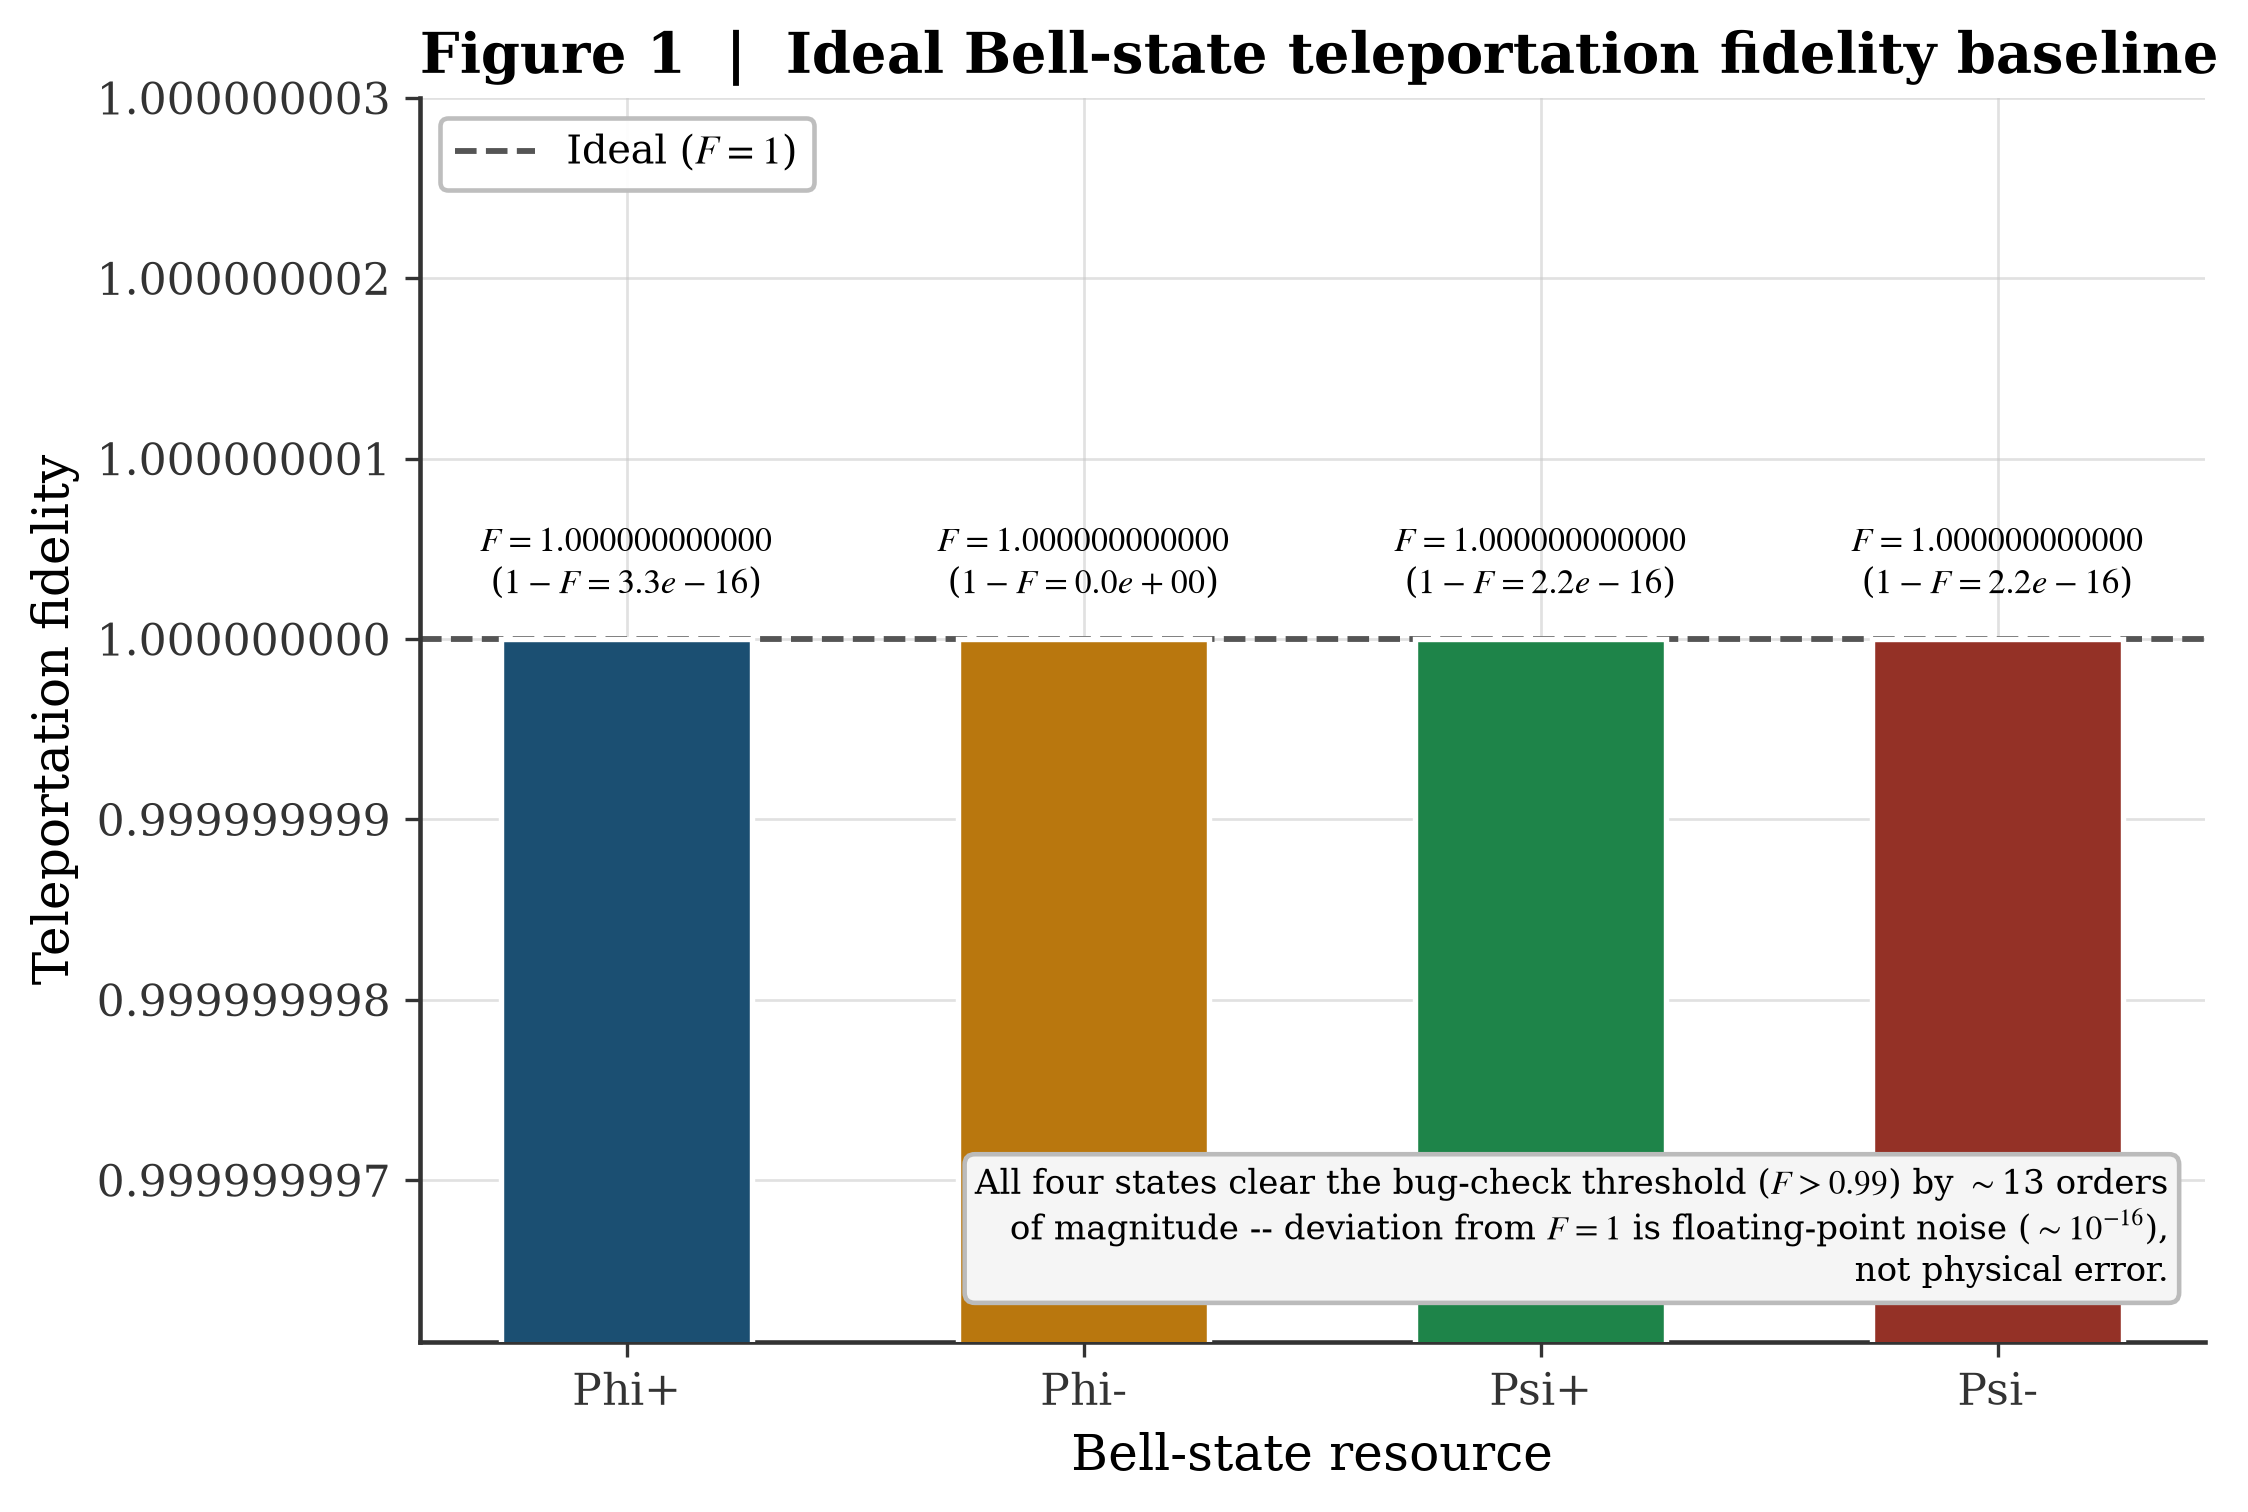
\includegraphics[width=0.6\linewidth]{figures/fig01_ideal_baseline.png}
\caption{Ideal (zero-noise) teleportation fidelity for all four Bell states.}
\label{fig:stage1}
\end{figure}

\begin{figure}[H]
\centering
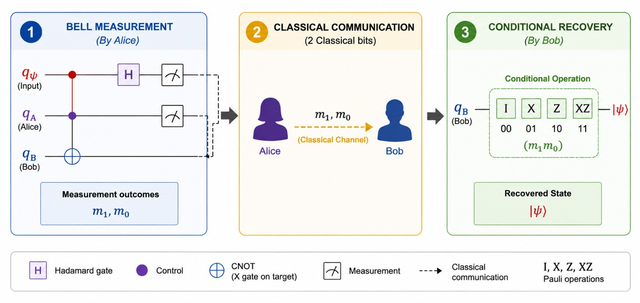
\includegraphics[width=0.75\linewidth]{figures/fig5_teleportation_protocol_diagram.png}
\caption{Schematic of the three-qubit teleportation protocol used throughout this study.}
\label{fig:protocol}
\end{figure}

\subsection{Stage 2: Effect of the four noise channels}
\label{sec:results-stage2}

\subsubsection{Structural result for the three Pauli channels}

Bit-flip, phase-flip, and depolarizing noise are built purely from Pauli operators. For this family it is a known theoretical result \citep{usher2017} that injecting the channel on the input qubit before an otherwise-ideal protocol gives the same output fidelity as injecting it directly on the Bell pair. This was confirmed numerically: the two placements agreed to floating-point precision (maximum difference $\approx10^{-15}$) for all three channels, across every Bell state and every noise strength tested. Consequently, for bit-flip, phase-flip, and depolarizing noise, \emph{all four Bell states produce mathematically identical fidelity} under this noise-injection scheme, and this particular way of injecting noise cannot distinguish the robustness of different Bell states.

\subsubsection{Amplitude-damping is the exception}

Amplitude-damping is not built from Pauli operators and is non-unital (it has a fixed point at $\ket0$), so the input-qubit/Bell-pair equivalence above does not apply to it. When amplitude-damping was applied directly to the Bell pair --- the physically correct placement for a Bell-state-robustness study, since the resource state is what actually experiences hardware noise --- the result differed substantially from the input-qubit version (maximum $|\Delta F|=0.74$ across all states, Bell states, and $p$, far above sampling noise). Unlike the three Pauli channels, the Bell-pair version of amplitude-damping is genuinely Bell-state-dependent: at $p=0.75$, fidelity ranges from $F=0.7033$ ($\Phi^+$) to $F=0.7168$ ($\Psi^-$), a spread of about $0.04$. Amplitude-damping is therefore the one channel in Stage~2 where a genuine Bell-state-dependent signal appears, once modeled correctly on the Bell pair rather than the input qubit.

\begin{figure}[H]
\centering
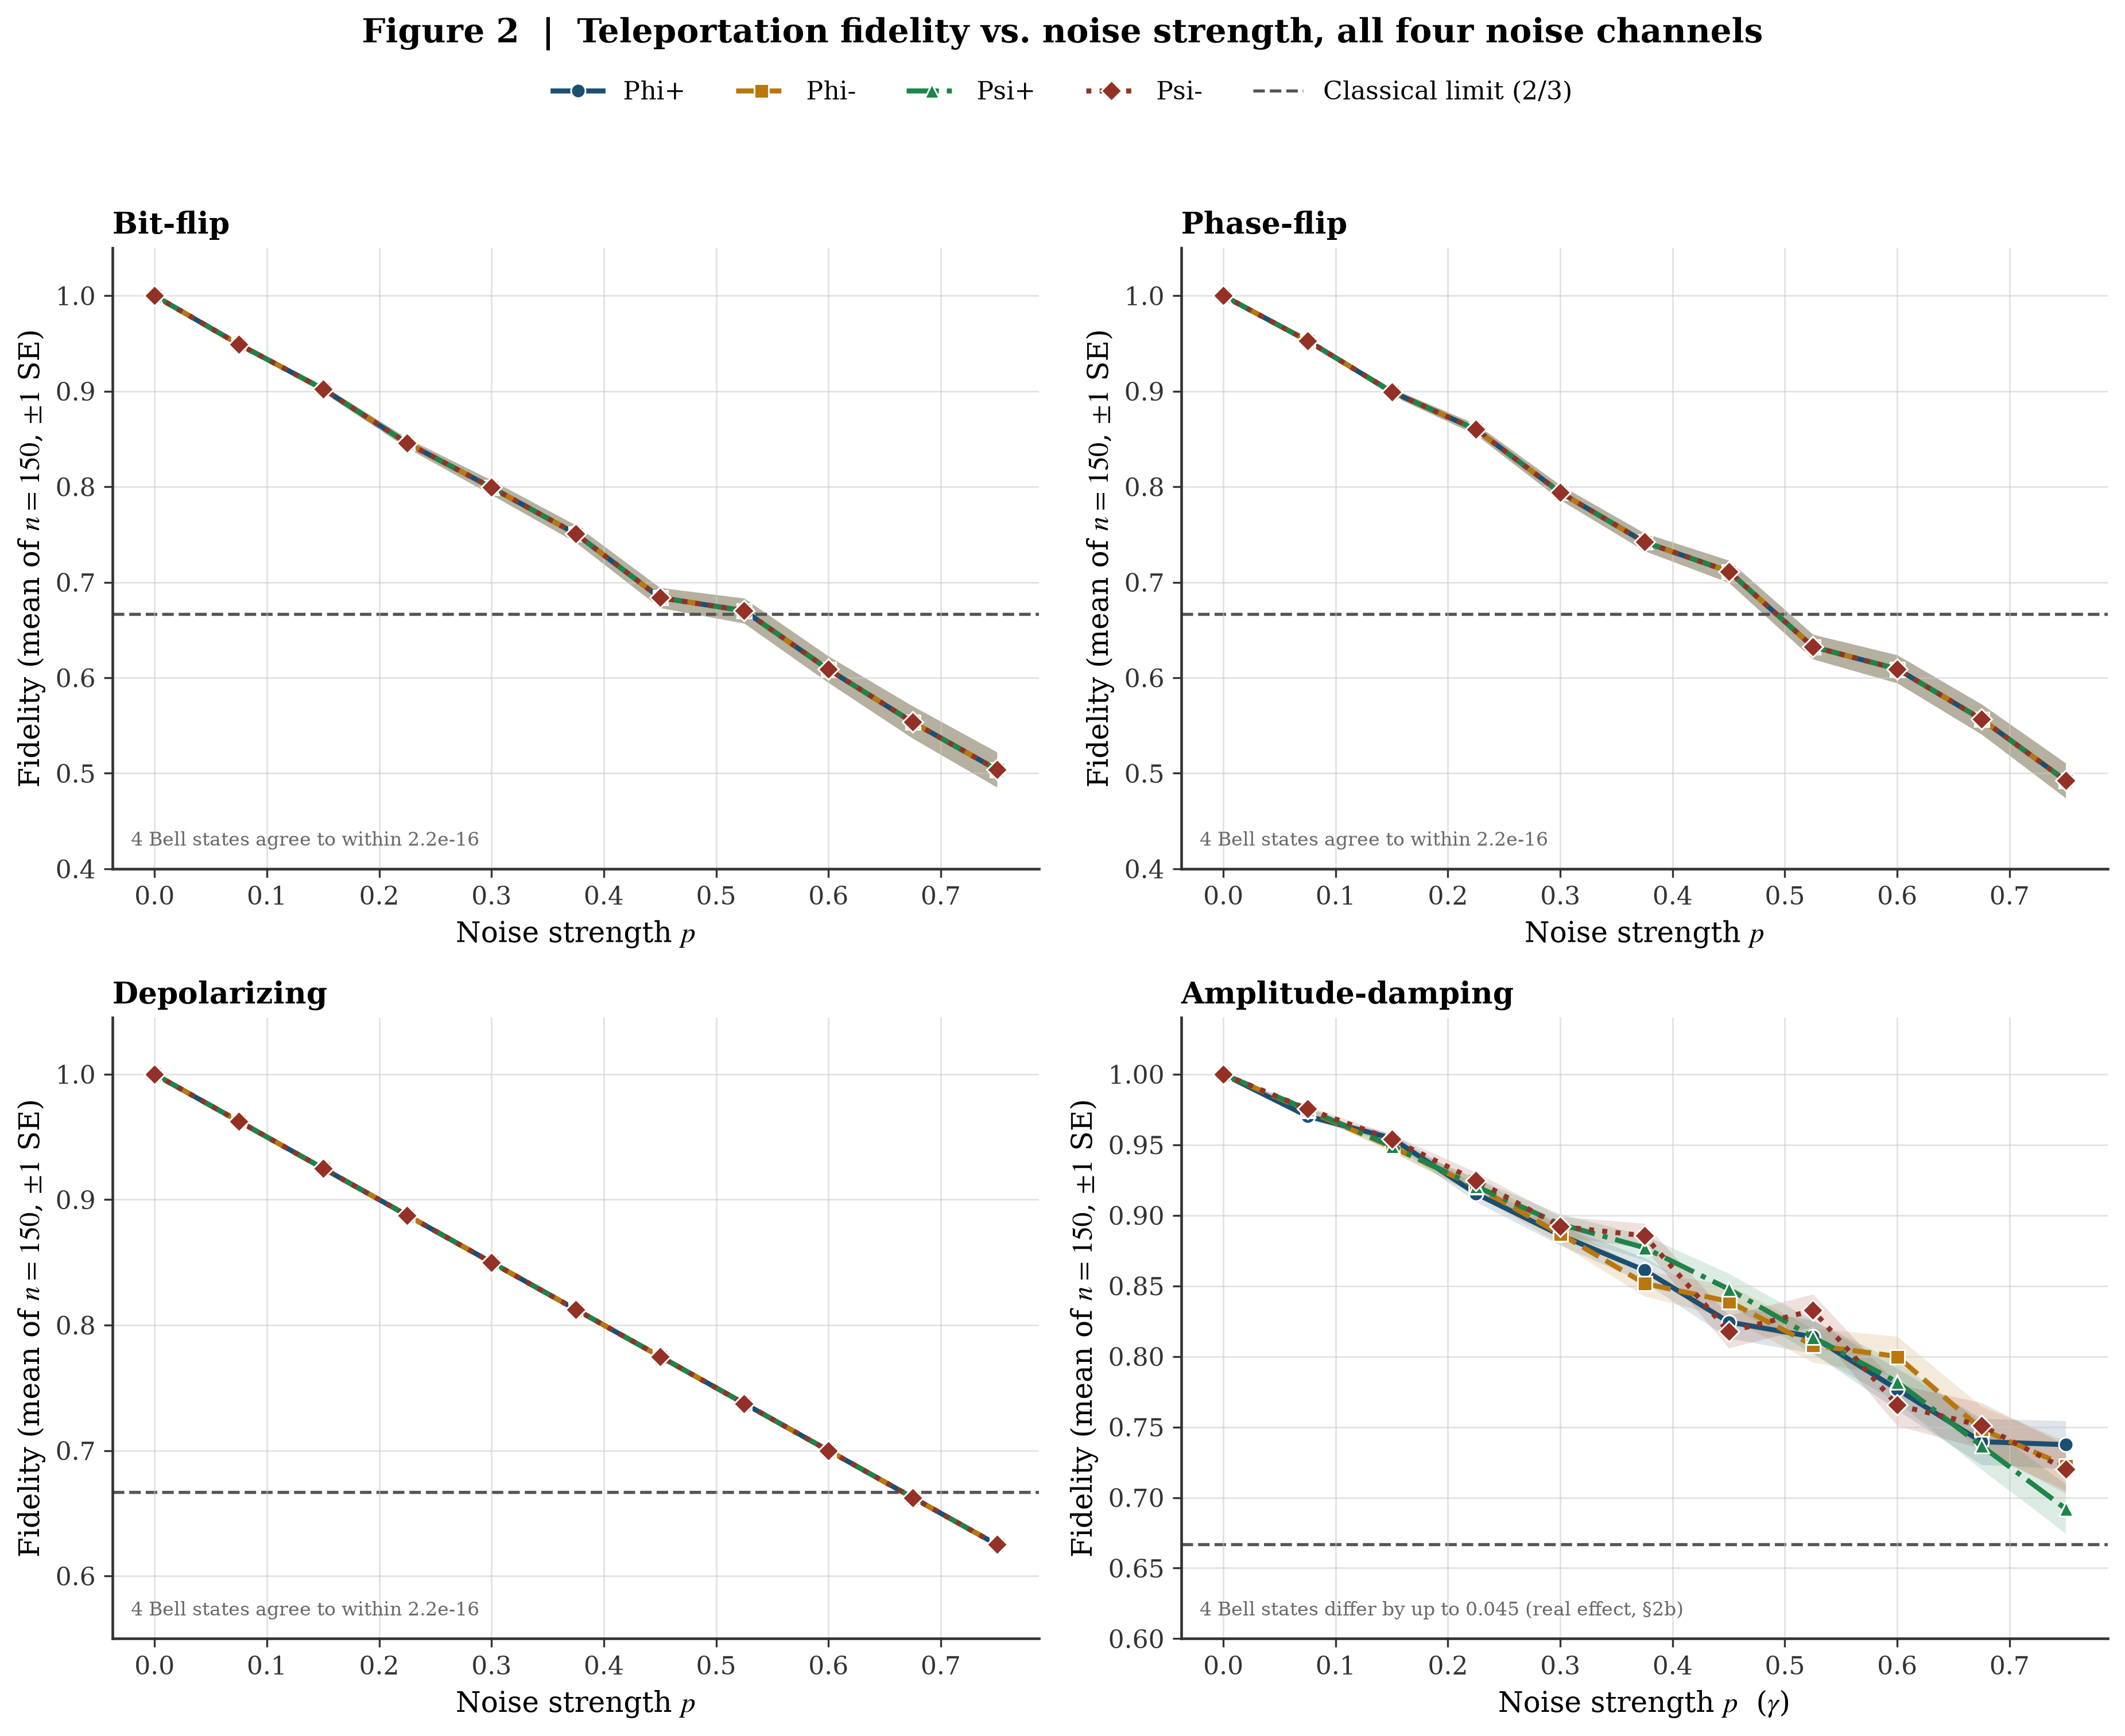
\includegraphics[width=0.92\linewidth]{figures/fig02_channel_grid.png}
\caption{Teleportation fidelity vs.\ noise strength for all four noise channels, one panel per channel, all four Bell-state curves overlaid with $\pm1$ standard-error bands (Haar-averaged, $n=150$). The three Pauli channels (top row, bottom-left) show the four Bell-state curves exactly on top of each other; amplitude-damping (bottom-right) is the one channel where they visibly separate.}
\label{fig:stage2grid}
\end{figure}

\begin{figure}[H]
\centering
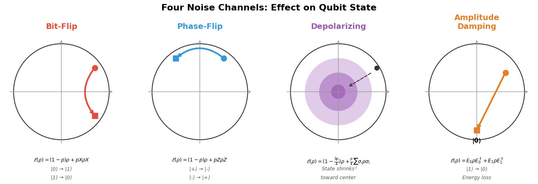
\includegraphics[width=0.7\linewidth]{figures/fig8_noise_channels_bloch_sphere.png}
\caption{Bloch-sphere representation of the four noise channels acting on a single qubit.}
\label{fig:bloch}
\end{figure}

\subsubsection{Channel ranking}

The four channels do not damage fidelity at the same rate. Initial expectations, based on the literature, were that depolarizing and amplitude-damping would degrade fidelity fastest; the simulated data show the opposite. Amplitude-damping is the gentlest channel, depolarizing is the second-gentlest, and bit-flip and phase-flip are the most damaging, becoming numerically indistinguishable from each other once averaged over random states.

This is explained by geometry: bit-flip and phase-flip each push every qubit state in one fixed direction, so states that align badly with that direction lose the most fidelity, and averaged over all possible states this is worse than depolarizing (which spreads the same error across three directions, allowing some cancellation) or amplitude-damping (which leaves $\ket0$ untouched, so many input states barely lose anything).

\begin{table}[H]
\centering
\caption{Channel ranking by fidelity at $p=0.75$ (Haar-averaged, $n=150$).}
\label{tab:ranking}
\begin{tabular}{clc}
\toprule
Rank & Channel & Fidelity at $p=0.75$ \\
\midrule
1 (worst) & Phase-flip & 0.4925 \\
2 & Bit-flip & 0.5039 \\
3 & Depolarizing & 0.6250 \\
4 (best) & Amplitude-damping & 0.7110 (avg.\ of Bell-state-dependent values, 0.7033--0.7168) \\
\bottomrule
\end{tabular}
\end{table}

\begin{figure}[H]
\centering
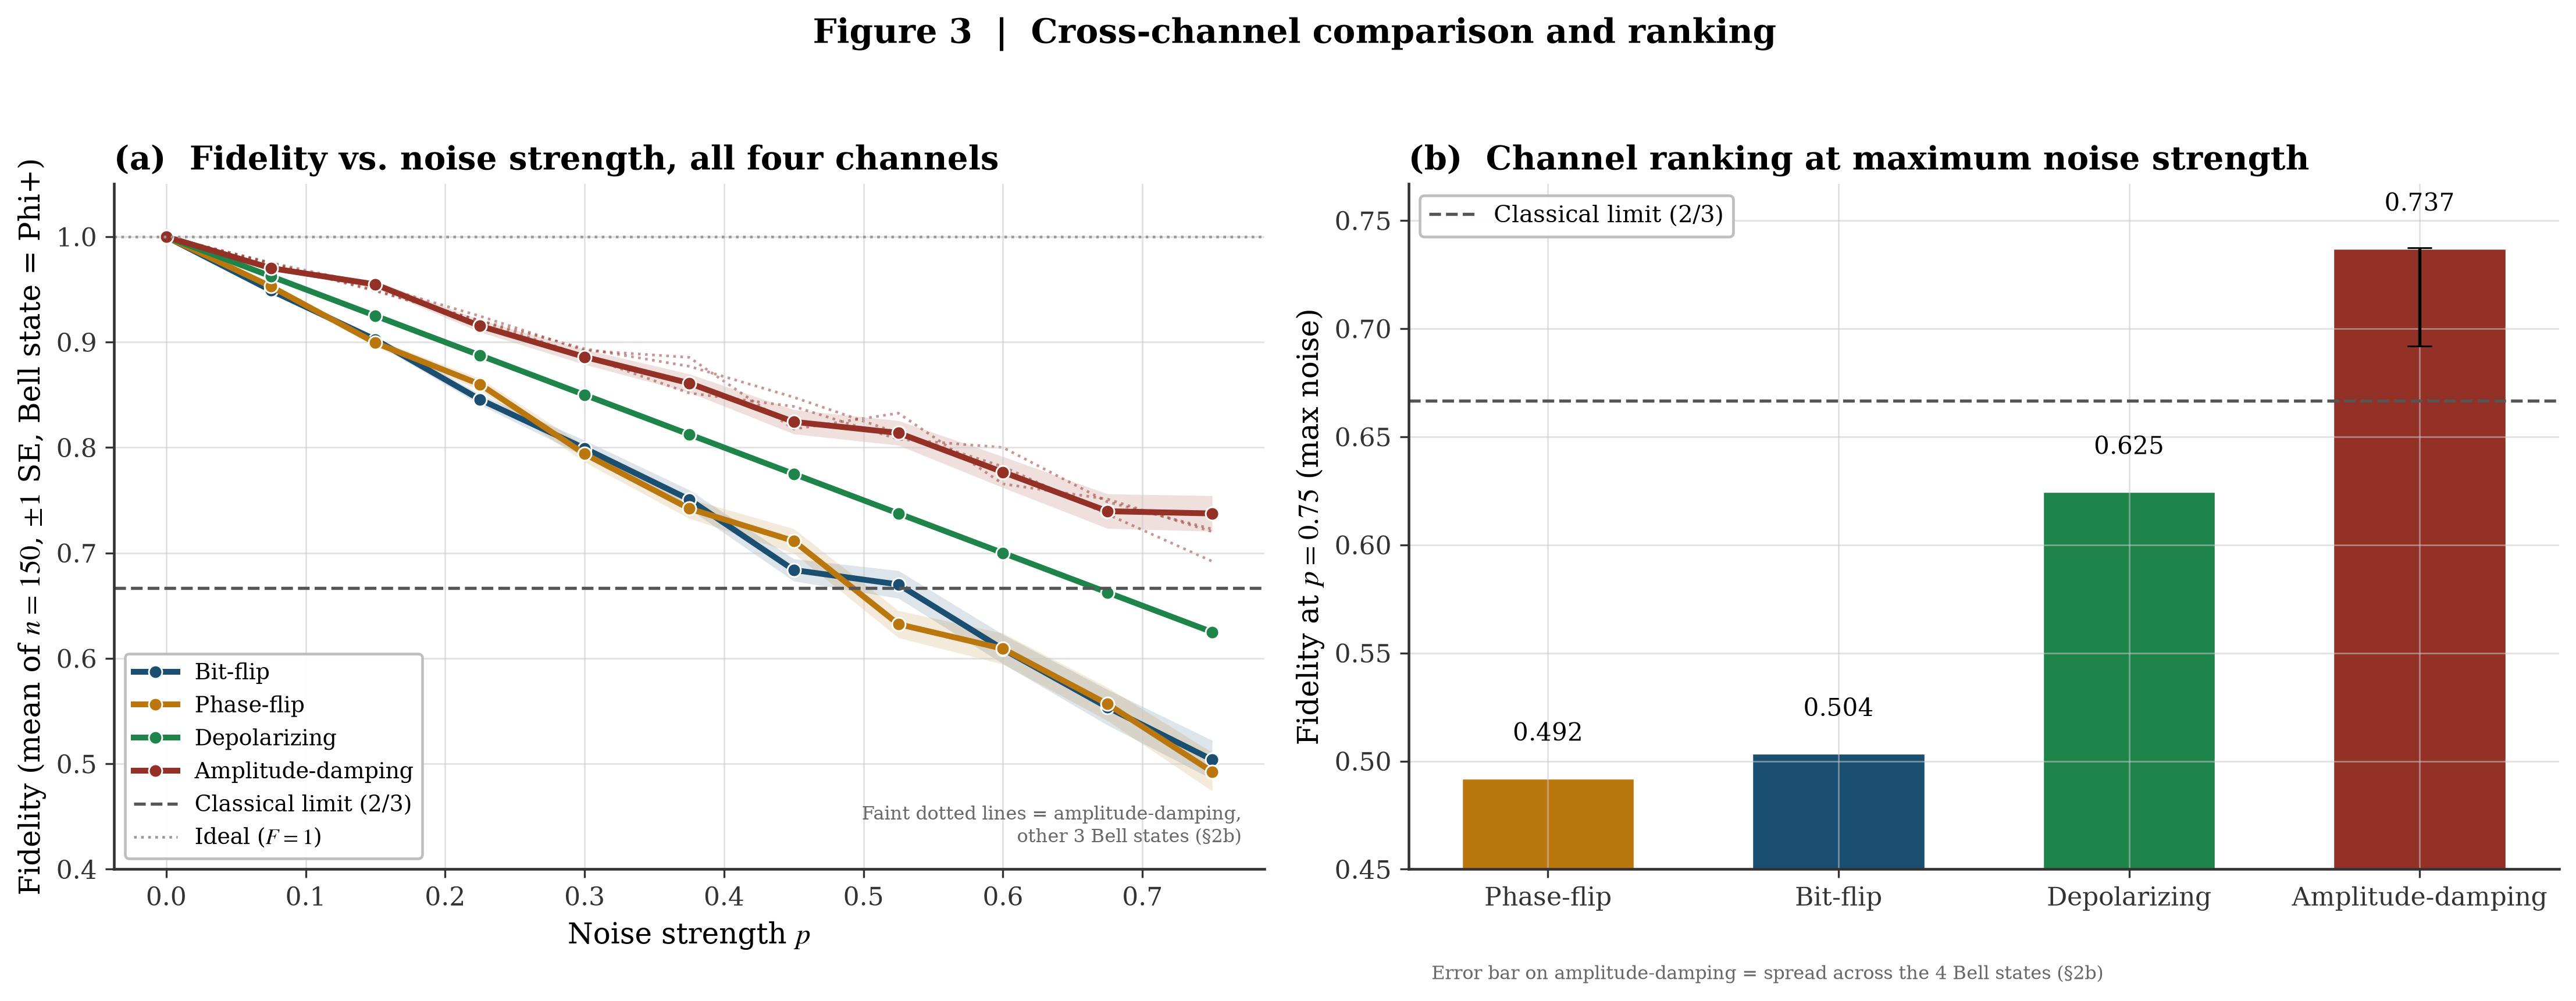
\includegraphics[width=0.98\linewidth]{figures/fig03_channel_comparison_and_ranking.png}
\caption{Stage 2 results for the representative Bell state $\Phi^+$: (a) fidelity vs.\ noise strength for all four channels, with $\pm1$ standard-error bands (faint dotted lines show the other three Bell states for amplitude-damping only, \S\ref{sec:results-stage2}); (b) channel ranking at maximum noise strength $p=0.75$, with the amplitude-damping error bar showing its spread across Bell states. The dashed line marks the classical limit $F_{\text{classical}}=2/3$.}
\label{fig:stage2}
\end{figure}

\subsection{Stage 3: Routing noise --- natural vs.\ forced-SWAP layout}
\label{sec:results-stage3}

\textbf{Calibration-based prediction:} Natural $F\approx0.9847$, Forced $F\approx0.9617$ --- a predicted drop of about $2.33\%$.

\textbf{Actual simulated result} (pooled across all four Bell states, $n=160$ per layout): Natural $F=0.9643\pm0.0006$, Forced $F=0.9507\pm0.0007$ --- an actual drop of about $1.41\%$.

The observed drop came in smaller than both the calibration-based prediction and an original $\approx23\%$ order-of-magnitude estimate made at the proposal stage (which conflated per-gate error with total fidelity loss). This is because the calibration formula (Eq.~\eqref{eq:F-gatecount}) accounts only for two-qubit gate error: it does not credit the natural layout for anything else, and it does not penalize the forced layout for its extra circuit depth (23 transpiled layers vs.\ 13) or for baseline single-qubit and readout error that both layouts share roughly equally, which dilutes the gap between them (see Section~\ref{sec:discussion}).

The drop is statistically robust: the $z$-score for the pooled comparison is $14.70$, well past the conventional two-standard-deviation threshold for significance. As in Stage~2, all four Bell states behaved essentially identically within each layout. The single lowest-fidelity case across all eight combinations was $\Psi^-$ on the forced layout ($F=0.9498$), which was carried forward into Stage~4 for error mitigation.

\begin{table}[H]
\centering
\caption{Fidelity for all eight (Bell state, layout) combinations, $n=40$ random input states each, 2048 shots per circuit.}
\label{tab:stage3-full}
\begin{tabular}{lccc}
\toprule
Bell state & Layout & Mean fidelity & Std.\ error \\
\midrule
$\Phi^+$ & Natural & 0.9645 & 0.0013 \\
$\Phi^+$ & Forced  & 0.9517 & 0.0013 \\
$\Phi^-$ & Natural & 0.9645 & 0.0013 \\
$\Phi^-$ & Forced  & 0.9509 & 0.0014 \\
$\Psi^+$ & Natural & 0.9642 & 0.0013 \\
$\Psi^+$ & Forced  & 0.9506 & 0.0013 \\
$\Psi^-$ & Natural & 0.9642 & 0.0013 \\
$\Psi^-$ & Forced  & \textbf{0.9498} (lowest of all 8) & 0.0014 \\
\bottomrule
\end{tabular}
\end{table}

\begin{figure}[H]
\centering
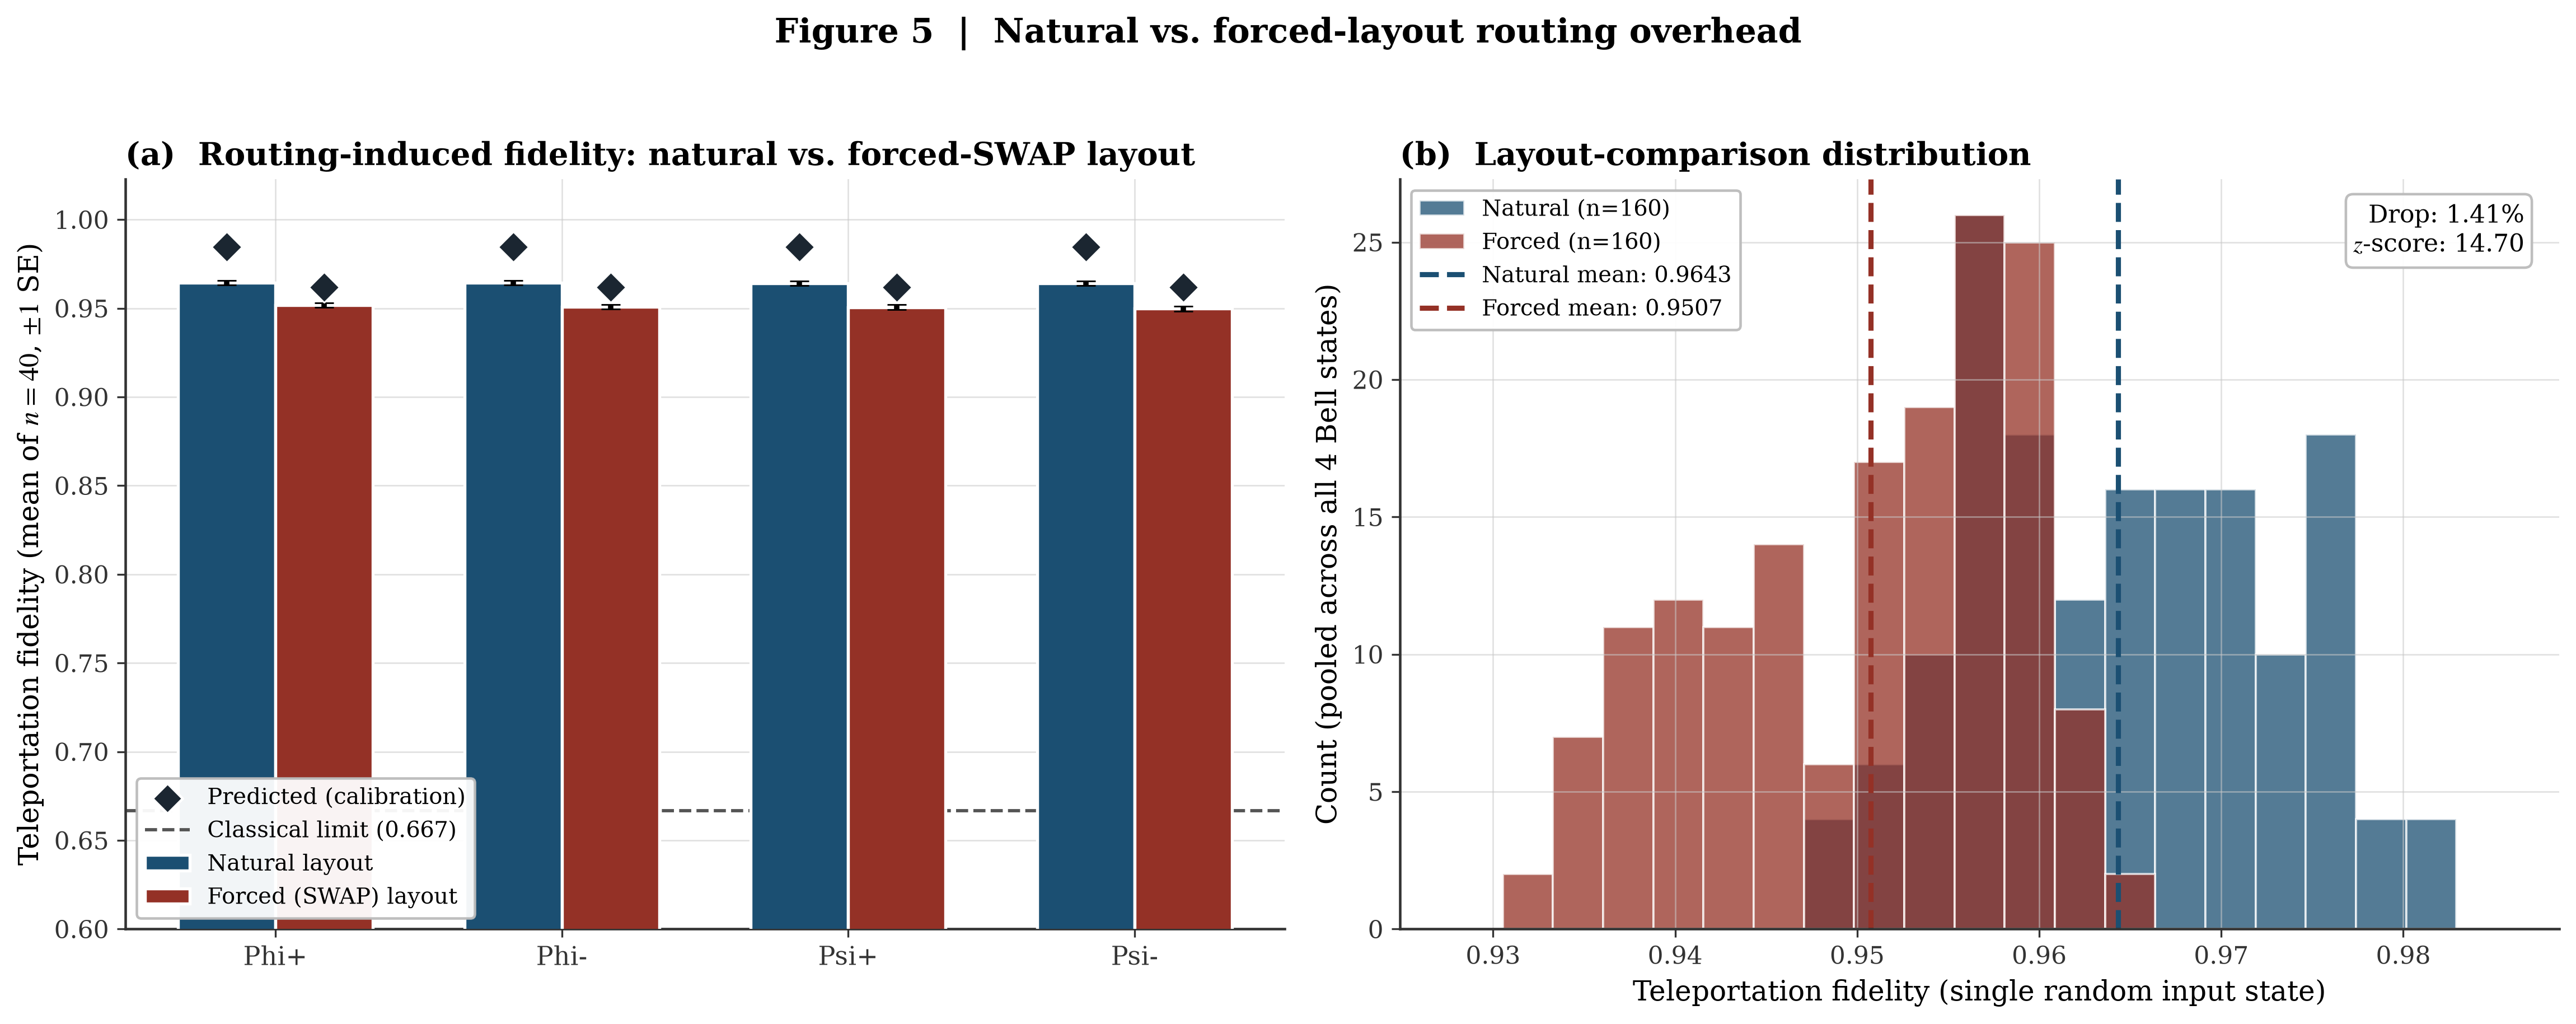
\includegraphics[width=0.85\linewidth]{figures/fig07_routing_natural_vs_forced.png}
\caption{Natural vs.\ forced-layout fidelity: (a) predicted (calibration-only, diamond markers) vs.\ simulated (full noise model, bars) fidelity per Bell state; (b) pooled fidelity distribution by layout, with the significance test result annotated.}
\label{fig:stage3}
\end{figure}

\begin{figure}[H]
\centering
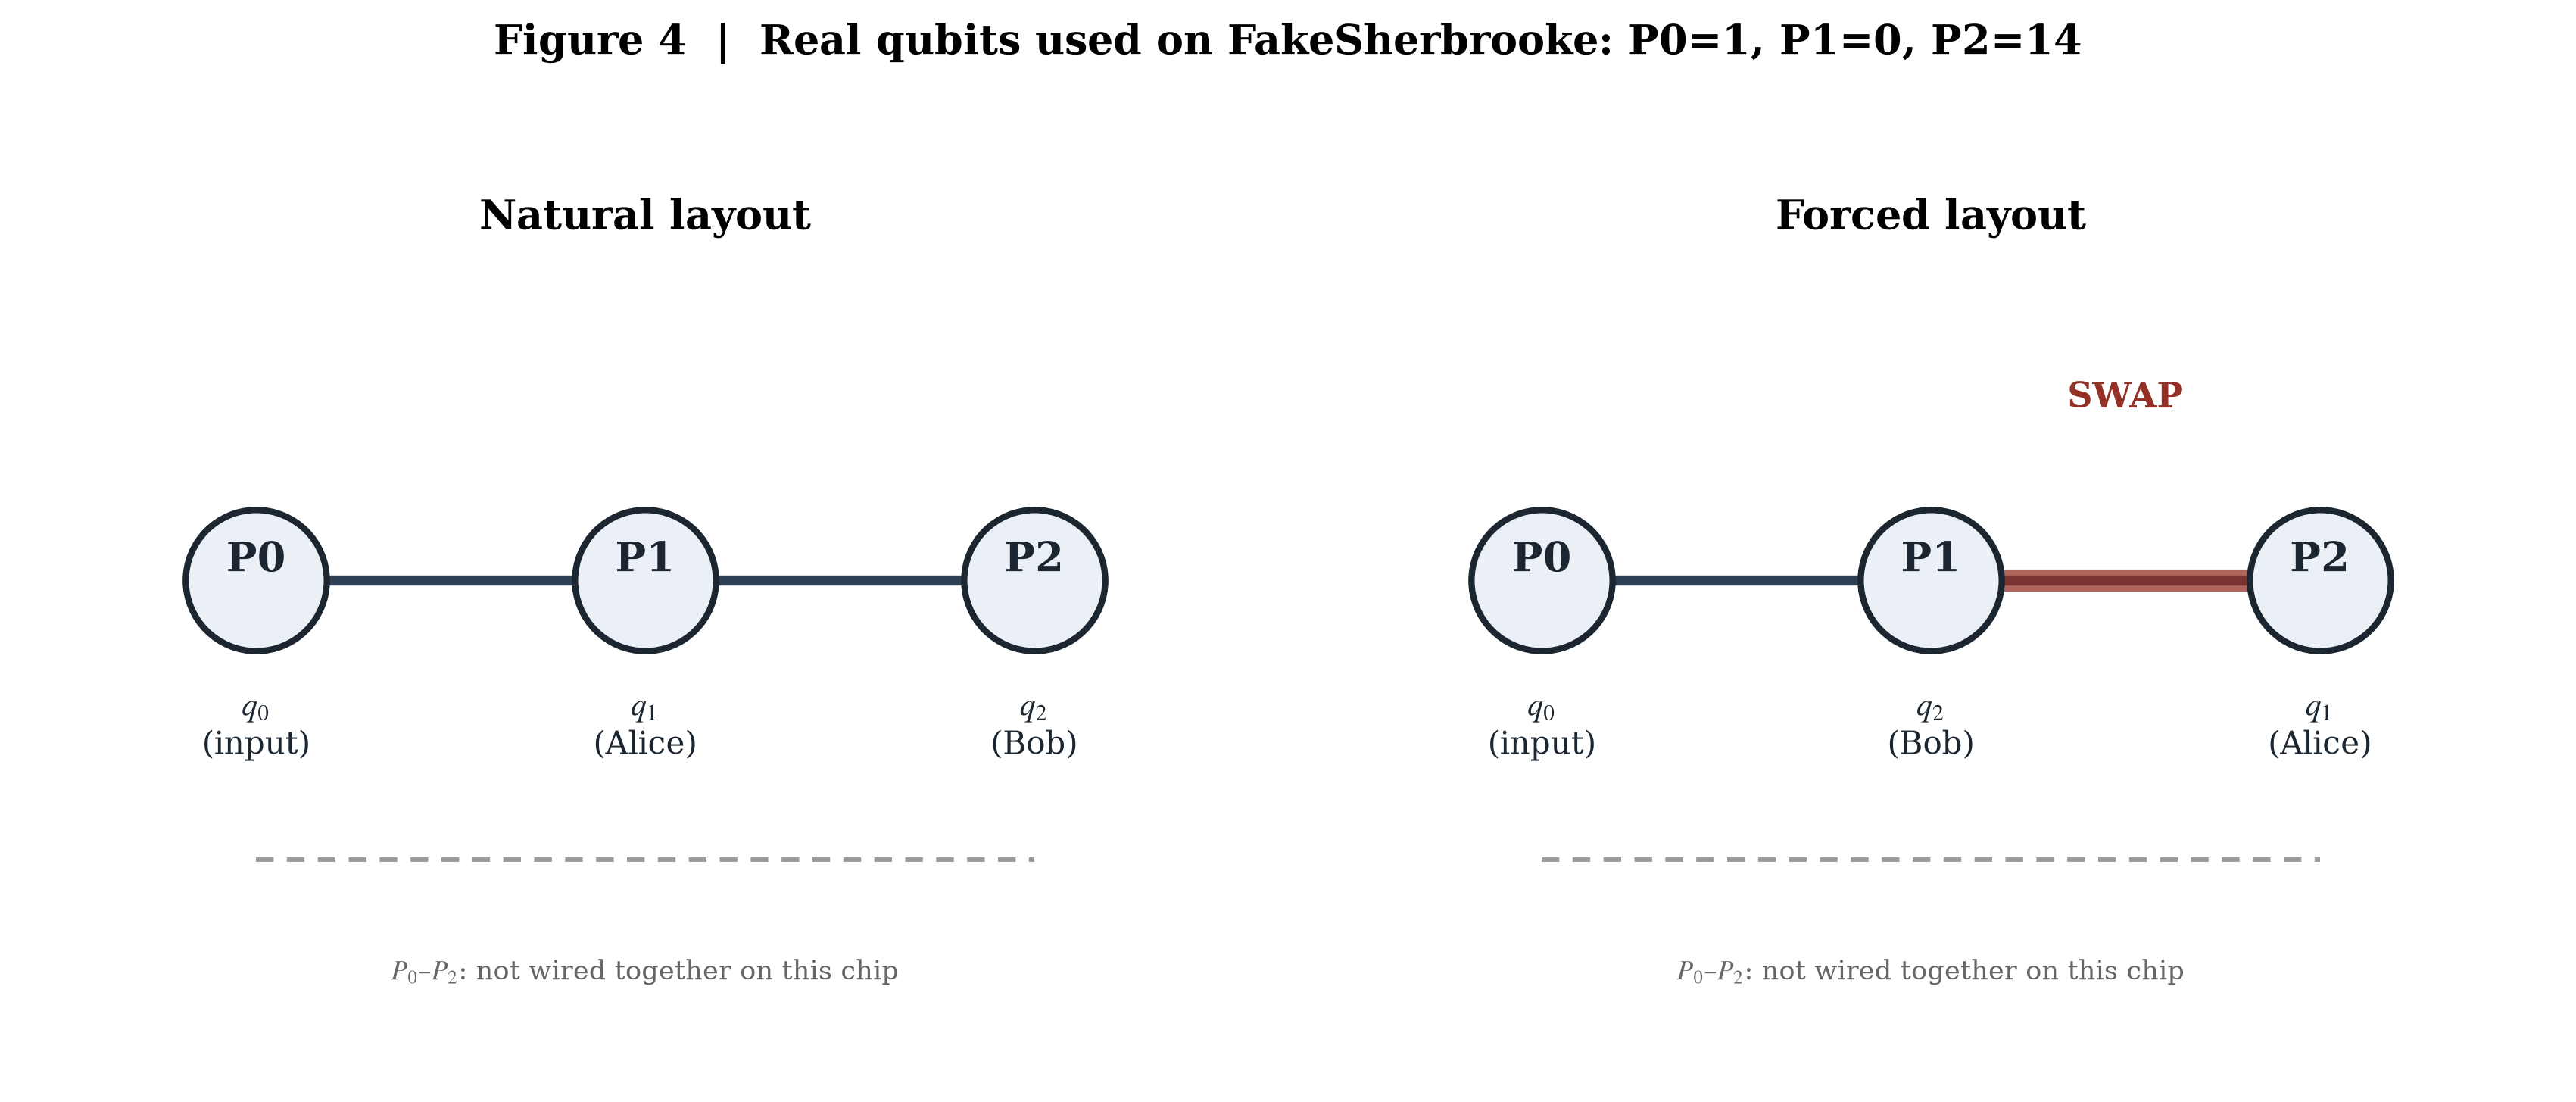
\includegraphics[width=0.92\linewidth]{figures/fig05_qubit_role_diagram.png}
\caption{The three physically adjacent qubits used on \texttt{FakeSherbrooke} ($P_0$--$P_1$--$P_2$) and how the logical roles $q_0$ (input), $q_1$ (Alice), $q_2$ (Bob) map onto them in the natural layout (no SWAP needed) versus the forced layout (SWAP inserted on the $P_1$--$P_2$ edge).}
\label{fig:qubitrole}
\end{figure}

\begin{figure}[H]
\centering
\begin{subfigure}[b]{0.48\linewidth}
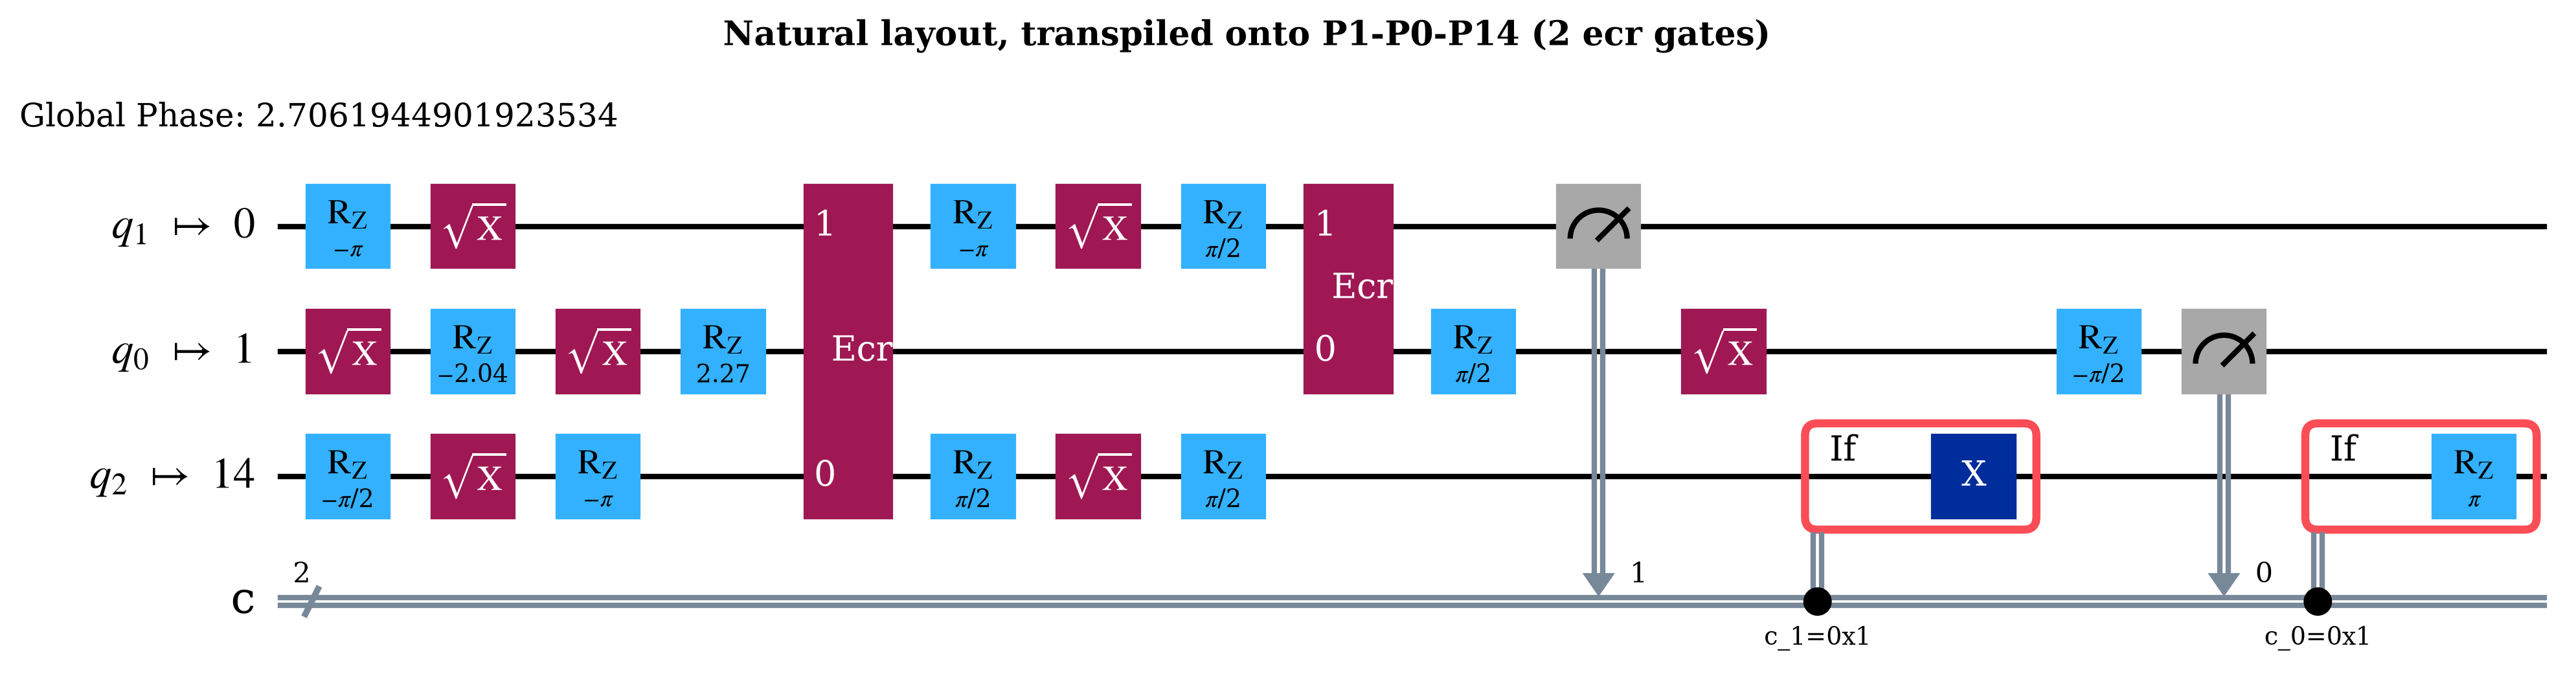
\includegraphics[width=\linewidth]{figures/fig06a_natural_circuit_transpiled.png}
\caption{Natural layout: 2 \texttt{ecr} gates.}
\end{subfigure}
\hfill
\begin{subfigure}[b]{0.48\linewidth}
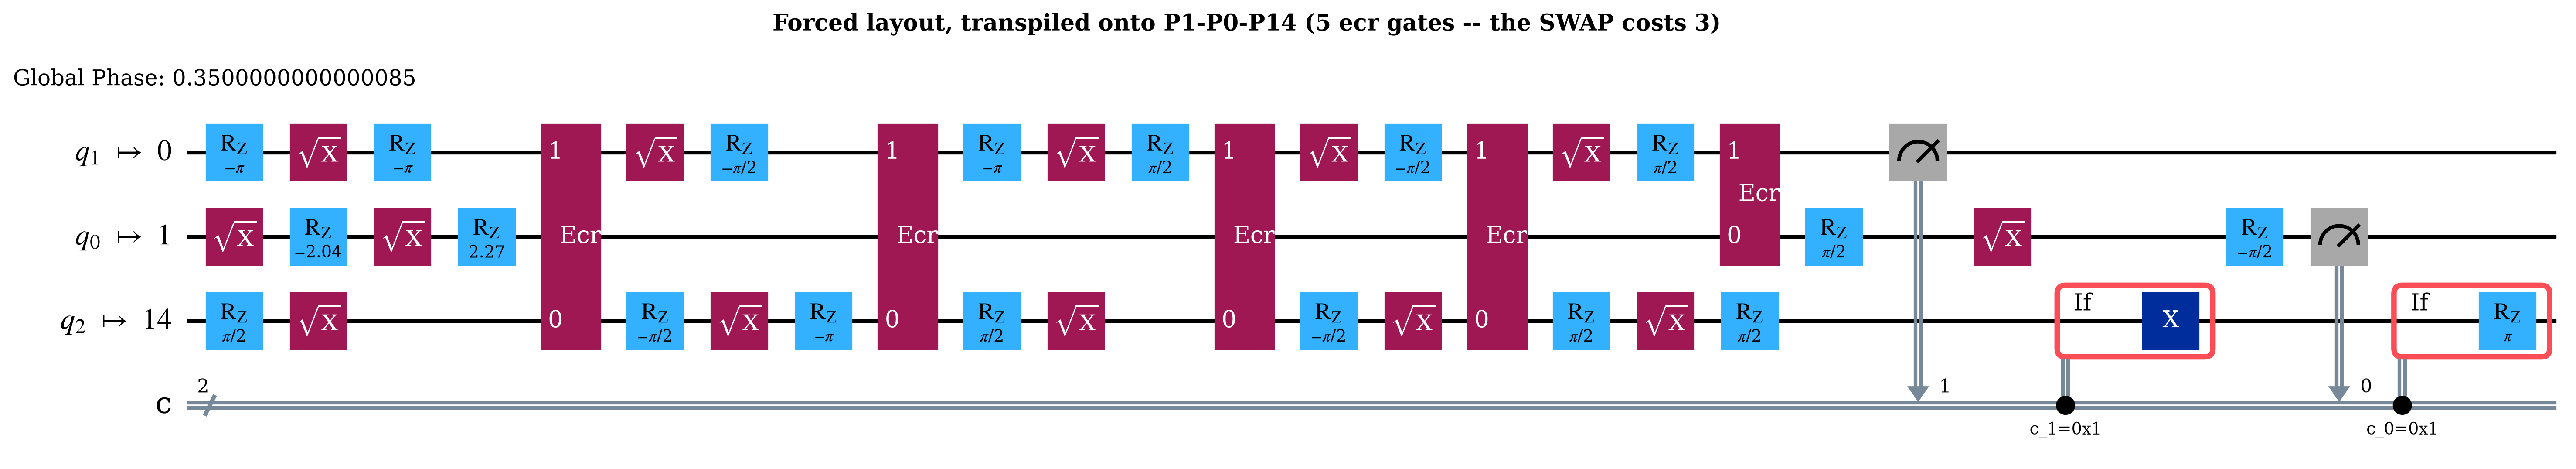
\includegraphics[width=\linewidth]{figures/fig06b_forced_circuit_transpiled.png}
\caption{Forced layout: 5 \texttt{ecr} gates (the extra SWAP costs 3).}
\end{subfigure}
\caption{Transpiled circuits on \texttt{FakeSherbrooke} for the natural and forced qubit layouts.}
\label{fig:circuits}
\end{figure}

\subsection{Stage 4: Zero-noise extrapolation}

Fidelity decreased smoothly as the fold scale increased (Table~\ref{tab:zne}), confirming that folding correctly injects extra real noise without changing the underlying logical circuit. The linear extrapolation recovered roughly 2.3 percentage points of fidelity (from $0.9476$ to $0.9701$) relative to the unmitigated forced-layout result. The quadratic check landed close to the linear estimate ($0.9723$ vs.\ $0.9701$), with no sign of the extrapolation overshooting (the estimated fidelity never exceeds 1).

\begin{table}[H]
\centering
\caption{ZNE fold-scale fidelities and extrapolated results for $\Psi^-$, forced layout.}
\label{tab:zne}
\begin{tabular}{lc}
\toprule
Fold scale & Fidelity \\
\midrule
$1\times$ (unmitigated) & 0.9476 \\
$3\times$ & 0.9025 \\
$5\times$ & 0.8630 \\
Linear ZNE (extrapolated, using $1\times$ \& $3\times$) & \textbf{0.9701} \\
Quadratic check (using all three points) & 0.9723 \\
\bottomrule
\end{tabular}
\end{table}

The ZNE result ($0.9701$) is not directly comparable to Stage 3's natural-layout average ($0.9643$), even though it is slightly higher: ZNE only extrapolates away the noise from the folded two-qubit gates; it does not remove the single-qubit and readout error present in every case, including the natural layout, which still carries two real, unmitigated two-qubit gates of its own (Section~\ref{sec:discussion}).

\begin{figure}[H]
\centering
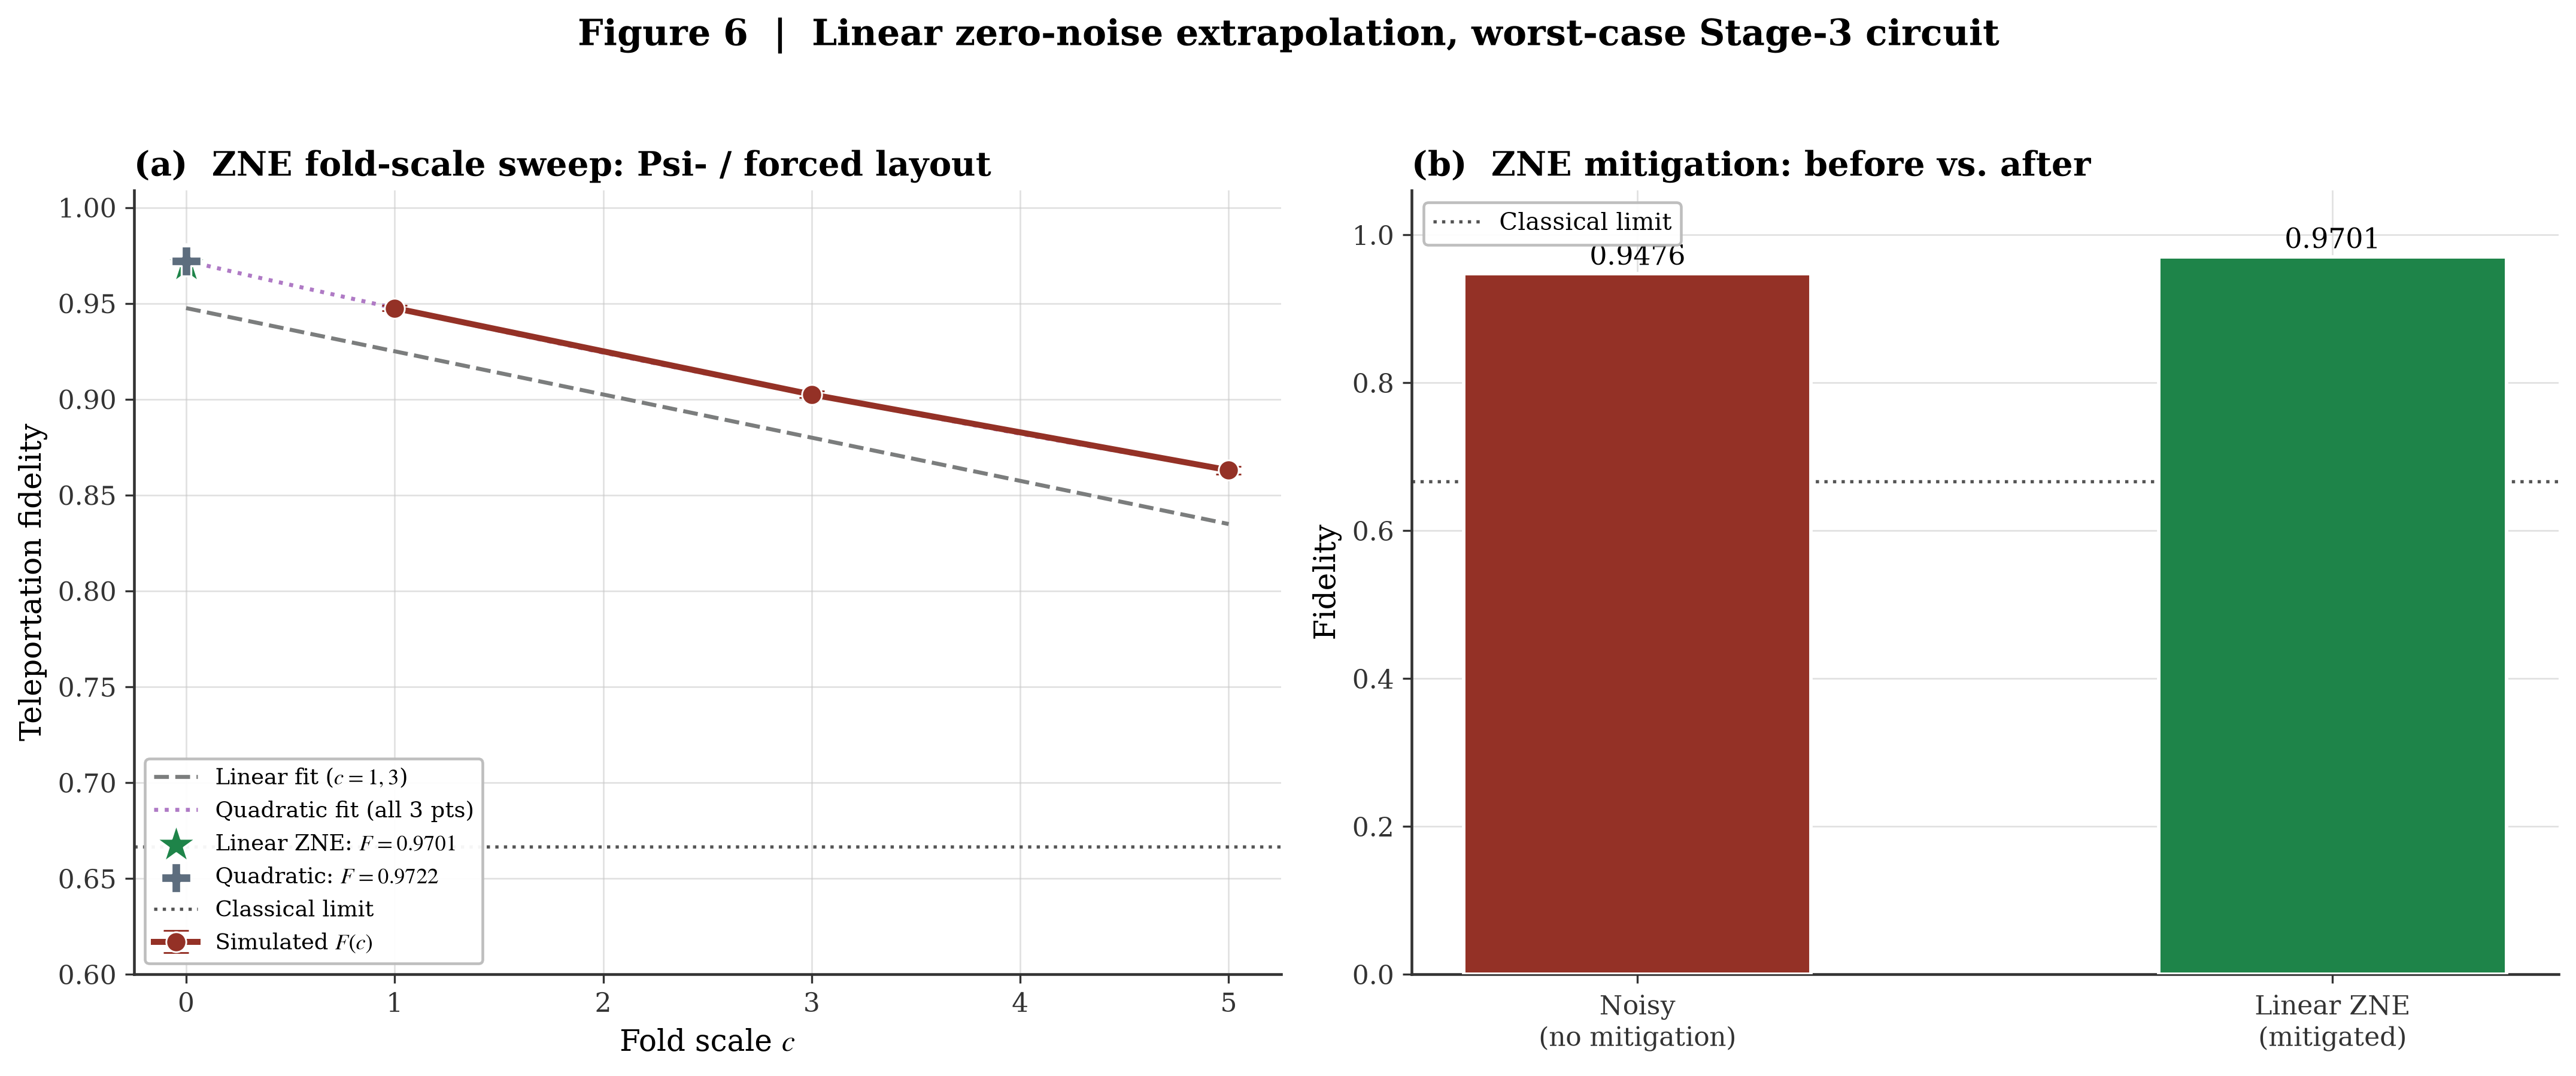
\includegraphics[width=0.85\linewidth]{figures/fig08_zne_foldscale_and_mitigation.png}
\caption{Fidelity vs.\ fold scale, with linear ZNE extrapolation to zero noise, for the worst-performing Stage 3 case ($\Psi^-$, forced layout).}
\label{fig:stage4}
\end{figure}

\section{Discussion: Reconciling the Calibration Prediction with the Simulation Result}
\label{sec:discussion}

\subsection{Gate errors and the calibration snapshot}

A gate error is the probability that a quantum gate fails to perform its intended transformation. For the two-qubit (\texttt{ecr}) gates used on IBM hardware in this study, the \texttt{FakeSherbrooke} calibration snapshot gives per-edge error rates of $0.7494\%$ (edge $P_0$--$P_1$) and $0.7845\%$ (edge $P_1$--$P_2$). These values come from measurements on a real IBM chip and, being reported as a single number, aggregate contributions from multiple underlying physical noise sources. The two edges differ because qubit pairs differ physically in isolation from environmental noise, calibration quality, and fabrication.

\subsection{The simplified calibration model}

The calibration-only prediction used the standard multiplicative model of Eq.~\eqref{eq:F-gatecount}:
\begin{align}
\text{Natural (2 gates):}\quad & F=(1-0.007845)\times(1-0.007494)=0.9847,\\
\text{Forced (5 gates):}\quad & F=(1-0.007845)^4\times(1-0.007494)=0.9617.
\end{align}
This gives a predicted drop of $2.33\%$.
This model, standard in the literature for a circuit with $l$ two-qubit gates each with error $p$ ($F\approx(1-p)^l$), implicitly assumes: noise arises only from two-qubit gates; each gate's error is independent and multiplies; single-qubit gates and readout are perfect; there is no crosstalk; coherence times are infinite; circuit depth does not matter beyond gate count; and a SWAP is exactly three CNOTs with no extra overhead. The derivation is mathematically correct under these assumptions.

\subsection{Why the full simulation gives a smaller relative drop}

The full noisy simulation (\texttt{AerSimulator.from\_backend(FakeSherbrooke)}) automatically includes everything in the \texttt{FakeSherbrooke} noise model, not only two-qubit gate error: single-qubit gate error (\texttt{rz}, \texttt{sx} gates), readout error, and $T_1/T_2$ decoherence. These additional sources act as a shared baseline that reduces absolute fidelity in both layouts, roughly proportionally, because they are present in both layouts almost equally. Because that extra noise is shared rather than SWAP-specific, it dilutes the relative gap between the natural and forced layouts even though both layouts individually end up with lower absolute fidelity than the calibration-only model predicted. This is why the predicted drop ($2.33\%$) is larger than the simulated drop ($1.41\%$), even though the simulated absolute fidelities are lower than predicted in both cases. The correct description of the mechanism is that shared baseline noise dilutes a relative comparison, not that errors from different sources cancel out.

Several specific factors contribute to this baseline:
\begin{itemize}[leftmargin=1.5em]
\item \textbf{Single-qubit gate errors} (\texttt{rz}, \texttt{sx}): individually small (typically $0.01$--$0.05\%$) but numerous --- the natural-layout circuit uses roughly 7 \texttt{sx} and 11 \texttt{rz} gates, the forced-layout circuit roughly 13 \texttt{sx} and 18 \texttt{rz} gates --- and present in both layouts.
\item \textbf{Readout error}: real IBM readout errors are typically $0.5$--$1.5\%$ per qubit; the circuit performs two measurements per shot in both layouts, and because the mid-circuit measurement drives the classical correction step, a readout error can cause the wrong correction to be applied.
\item \textbf{Decoherence ($T_1/T_2$ relaxation)}: the forced layout has a transpiled circuit depth of 23 compared with 13 for the natural layout, so qubits in the forced layout spend more time exposed to decay while idling or waiting for gates to complete.
\item \textbf{Gate placement and scheduling}: the calibration formula treats every gate as equally costly regardless of when it occurs; in practice gates later in the circuit act on qubits that have already accumulated some decoherence, and the three SWAP-related CNOTs in the forced layout are not all on the same physical edge.
\end{itemize}

An approximate error budget, built by separately estimating the contribution of two-qubit gate error, single-qubit gate error, readout error, and decoherence, and calibrating those estimates against the observed absolute fidelities, reproduces the pattern seen in the simulation: absolute losses are somewhat higher than the two-qubit-only model suggests, while the relative drop between layouts is smaller, consistent with a shared baseline diluting the comparison.

\subsection{Comparison across models}

\begin{table}[H]
\centering
\caption{Comparison of models used to estimate routing-induced fidelity loss.}
\label{tab:model-comparison}
\begin{tabular}{lp{6.5cm}l}
\toprule
Model & What it accounts for & Result \\
\midrule
Hand-derived & SWAP identity, gate counting, simplified error multiplication & Natural: 2 gates, Forced: 5 gates \\
Calibration-based & Two-qubit gate error only & Predicted drop: 2.33\% \\
Full simulation & Two-qubit + single-qubit + readout + decoherence + circuit depth & Observed drop: 1.41\% \\
\bottomrule
\end{tabular}
\end{table}

This progression --- a simplified model, tested against a fuller physical model, with the discrepancy explained rather than eliminated --- reflects standard practice when validating an analytic estimate against simulation: the full simulation was not missing anything that needed to be added after the fact, since the \texttt{FakeBackend} noise model already included single-qubit error, readout error, decoherence, and (to the extent modeled by the backend) crosstalk; only the hand-derived calibration formula was a deliberately simplified estimate.

\subsection{Why the ZNE result exceeds the natural-layout average}

The ZNE-mitigated fidelity ($0.9701$) is slightly higher than the natural layout's own average ($0.9643$). This follows directly from what ZNE targets: it extrapolates away only the two-qubit gate error from the gates that were folded (the SWAP-related gates in the forced layout). It does not remove single-qubit error, readout error, or decoherence. The natural layout still carries two real, unmitigated two-qubit gates plus the same baseline noise as every other case, so a forced-layout result with its SWAP-related two-qubit error fully extrapolated away is expected to land at or slightly above the natural layout's own noisy average --- a predictable consequence of what ZNE specifically targets, not an inconsistency in the results.

\subsection{Where each error factor appears across the four stages}

Stage~1 (ideal baseline) and Stage~2 (abstract Kraus-operator noise channels) do not involve any hardware noise model: Stage~1 has no noise at all, and Stage~2's noise is injected as an abstract channel with a single strength parameter, not via gate-level hardware error, readout error, or decoherence. Stage~3 (routing overhead) is the first stage where all real hardware error sources are present simultaneously, because it uses a full calibrated backend simulation rather than an abstract channel. Stage~4 (ZNE) inherits the same backend noise model as Stage~3, with the addition that the folded two-qubit gate error is deliberately scaled up across the three fold levels.

\begin{table}[H]
\centering
\caption{Presence of each error factor across the four stages.}
\label{tab:error-factors}
\resizebox{\textwidth}{!}{%
\begin{tabular}{lcccc}
\toprule
Error factor & Stage 1 & Stage 2 & Stage 3 & Stage 4 \\
\midrule
Two-qubit gate error & --- & --- & Primary factor & Folded / scaled \\
Single-qubit gate error & --- & --- & Background & Background \\
Readout error & --- & --- & Background & Background \\
Decoherence ($T_1/T_2$) & --- & Abstract (amplitude-damping only) & Physical & Physical \\
Crosstalk & --- & --- & Possible & Possible \\
Circuit depth effects & --- & --- & Emerges (23 vs.\ 13) & Emerges \\
SPAM errors & --- & --- & Background & Background \\
Pauli vs.\ non-unital structure & --- & Structural (Sec.~\ref{sec:results-stage2}) & --- & --- \\
\bottomrule
\end{tabular}%
}
\end{table}

\section{Conclusion}

This study verified that a three-qubit teleportation circuit reconstructs an arbitrary input state with $F\approx1$ under zero noise for all four Bell states, confirming correct circuit implementation. Under three of the four abstract noise channels --- bit-flip, phase-flip, depolarizing --- all four Bell states behave identically, a structural consequence of how Pauli-type noise commutes through the protocol rather than a limitation of the analysis. Amplitude-damping is the exception: because it is non-unital, applying it correctly to the Bell pair (rather than the input qubit) reveals a genuine, if modest, Bell-state-dependent spread ($\approx0.04$ at $p=0.75$), making it the one channel where Bell-state robustness can be meaningfully compared. The channel ranking itself was a genuine surprise relative to initial literature-based expectations: amplitude-damping and depolarizing are gentler than bit-flip and phase-flip.

Once noise is tied to something Bell-state-preparation-specific --- real routing/SWAP overhead using real chip calibration data --- a genuine gap appears between the natural and forced layouts (about $1.41\%$ fidelity loss), and this gap is statistically significant ($z\approx14.70$), even though the four Bell states still perform near-identically within each layout. The calibration-only prediction ($2.33\%$ drop) overestimates the actual relative drop because it accounts for two-qubit gate error alone; the fuller simulation shows that single-qubit gate error, readout error, and decoherence form a shared baseline that dilutes the relative comparison between layouts, even as it lowers absolute fidelity in both. Linear ZNE recovers a meaningful share ($\approx2.3$ percentage points) of the fidelity lost to the forced layout's extra SWAP gate, without requiring a more complex extrapolation method; a quadratic cross-check confirms the linear estimate is not overshooting.

Taken together, routing overhead --- not Bell-state choice --- is the dominant hardware-limited error source identified in this study, and its impact is smaller in practice than a calibration-only estimate suggests once the full noise model is accounted for. Software-level mitigation such as ZNE recovers a meaningful share of that loss without any change to the underlying hardware, suggesting a practical, low-overhead path toward improving near-term quantum communication fidelity on fixed-connectivity NISQ devices.

\appendix

\section{Reduction of the General Noise Superoperator to the Pauli-Channel Form}
\label{app:reduction}

Starting from the general noisy-teleportation superoperator \citep[Eq.~8]{oh2002},
\begin{equation}
\mathcal{E}(\rho_{\text{out}}) = \Tr_{1,2}\left[U_{\text{tel}}\left(\mathcal{E}(\rho_{\text{in}})\otimes\rho_{\text{ent}}\right)U_{\text{tel}}^\dagger\right].
\label{eq:app-start}
\end{equation}
For a Pauli channel $\mathcal{E}(\rho)=(1-p)\rho+pA\rho A$:
\begin{align}
\mathcal{E}(\rho_{\text{out}}) &= \Tr_{1,2}\left[U_{\text{tel}}\left(\left((1-p)\rho_{\text{in}}+pA\rho_{\text{in}}A\right)\otimes\rho_{\text{ent}}\right)U_{\text{tel}}^\dagger\right] \label{eq:app1}\\
&= (1-p)\Tr_{1,2}\left[U_{\text{tel}}\left(\rho_{\text{in}}\otimes\rho_{\text{ent}}\right)U_{\text{tel}}^\dagger\right] + p\,\Tr_{1,2}\left[U_{\text{tel}}\left(A\rho_{\text{in}}A\otimes\rho_{\text{ent}}\right)U_{\text{tel}}^\dagger\right]. \label{eq:app2}
\end{align}
Since ideal teleportation transmits any input state perfectly:
\begin{equation}
\Tr_{1,2}\left[U_{\text{tel}}\left(\rho_{\text{in}}\otimes\rho_{\text{ent}}\right)U_{\text{tel}}^\dagger\right] = \rho_{\text{in}}, \qquad
\Tr_{1,2}\left[U_{\text{tel}}\left(A\rho_{\text{in}}A\otimes\rho_{\text{ent}}\right)U_{\text{tel}}^\dagger\right] = A\rho_{\text{in}}A.
\label{eq:app3}
\end{equation}
Therefore
\begin{equation}
\mathcal{E}(\rho_{\text{out}}) = (1-p)\rho_{\text{in}} + pA\rho_{\text{in}}A.
\label{eq:app-final}
\end{equation}
This reduction holds for any Pauli channel ($A\in\{X,Y,Z\}$). For the depolarizing channel, the sum over all three Pauli operators gives the corresponding expression. For amplitude-damping, which is not a Pauli channel, this reduction does not apply and the full Kraus-operator calculation of Section~\ref{sec:stage2-theory} is used instead.

\section*{Data and Code Availability}
The simulation code, Jupyter notebooks, and figure-generation scripts used in this study are available at:\\
\href{https://github.com/pallasArchive/Quantum-Teleportation-Robustness-of-Bell-Entangelled-Channel-with-Linear-ZNE}{github.com/pallasArchive/Quantum-Teleportation-Robustness-of-Bell-Entangelled-Channel-with-Linear-ZNE}

\bibliographystyle{unsrtnat}
\begin{thebibliography}{9}

\bibitem[Bennett et al.(1993)]{bennett1993}
C. H. Bennett, G. Brassard, C. Cr\'epeau, R. Jozsa, A. Peres, and W. K. Wootters,
``Teleporting an unknown quantum state via dual classical and Einstein-Podolsky-Rosen channels,''
\textit{Phys. Rev. Lett.}, vol.\ 70, no.\ 13, pp.\ 1895--1899, 1993.

\bibitem[Oh et al.(2002)]{oh2002}
S. Oh, S. Lee, and H. Lee,
``Fidelity of quantum teleportation through noisy channels,''
\textit{Phys. Rev. A}, vol.\ 66, no.\ 2, p.\ 022316, 2002.

\bibitem[Usher and Browne(2017)]{usher2017}
N. Usher and D. E. Browne,
``Noise in One-Dimensional Measurement-Based Quantum Computing,''
\textit{Quantum Information and Computation}, vol.\ 17, no.\ 15--16, pp.\ 1372--1397, 2017.
arXiv:1704.07298.

\bibitem[Hillmich et al.(2021)]{hillmich2021}
S. Hillmich, A. Zulehner, and R. Wille,
``Exploiting Quantum Teleportation in Quantum Circuit Mapping,''
in \textit{Proc.\ 26th Asia and South Pacific Design Automation Conference (ASP-DAC '21)}, Tokyo, Japan, 2021, pp.\ 792--797.
doi: 10.1145/3394885.3431604. arXiv:2011.07314.

\bibitem[Pina-Canelles et al.(2025)]{pina2025}
V. Pina-Canelles, A. Auer, and I. de Vega,
``Improving and benchmarking NISQ qubit routers,''
arXiv preprint arXiv:2502.03908, 2025.

\bibitem[Sohn et al.(2025)]{sohn2025}
H. Sohn, J. Jung, J. Park, H. Jang, L. E. A. Stehouwer, D. Degli Esposti, G. Scappucci, and D. Kim,
``Application of zero-noise-extrapolation-based quantum error mitigation to a silicon spin qubit,''
\textit{Phys. Rev. A}, vol.\ 112, p.\ 012408, 2025.

\bibitem[Nielsen(2002)]{nielsen2002}
M. A. Nielsen,
``A simple formula for the average gate fidelity of a quantum dynamical operation,''
\textit{Physics Letters A}, vol.\ 303, no.\ 4, pp.\ 249--252, 2002.

\bibitem[Rindell et al.(2023)]{rindell2023}
T. Rindell, B. Yenilen, N. Halonen, A. P\"onni, I. Tittonen, and M. Raasakka,
``Exploring the optimality of approximate state preparation quantum circuits with a genetic algorithm,''
\textit{Physics Letters A}, vol.\ 475, p.\ 128860, 2023. arXiv:2210.06411.

\end{thebibliography}

\end{document}
